\section{Longitudinal Connectivity {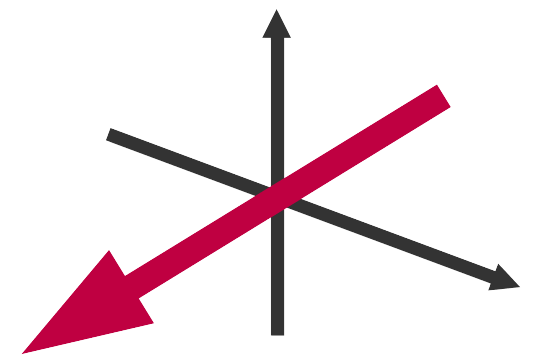
\includegraphics[height=15pt]{connectivity-x-small}}}

\subsection{Reservoir Sedimentation - Principles}

\begin{frame}{\secname\vspace{0.1cm}\\\textcolor{anthrazit!80!white}{\subsecname}}
	\begin{tikzpicture}
		\clip (0,0) rectangle (\paperwidth,\paperheight);
		\onslide<1->{
		\begin{scope}
				\node[anchor=south west, xshift=0.0\paperwidth, yshift=0.48\paperheight] {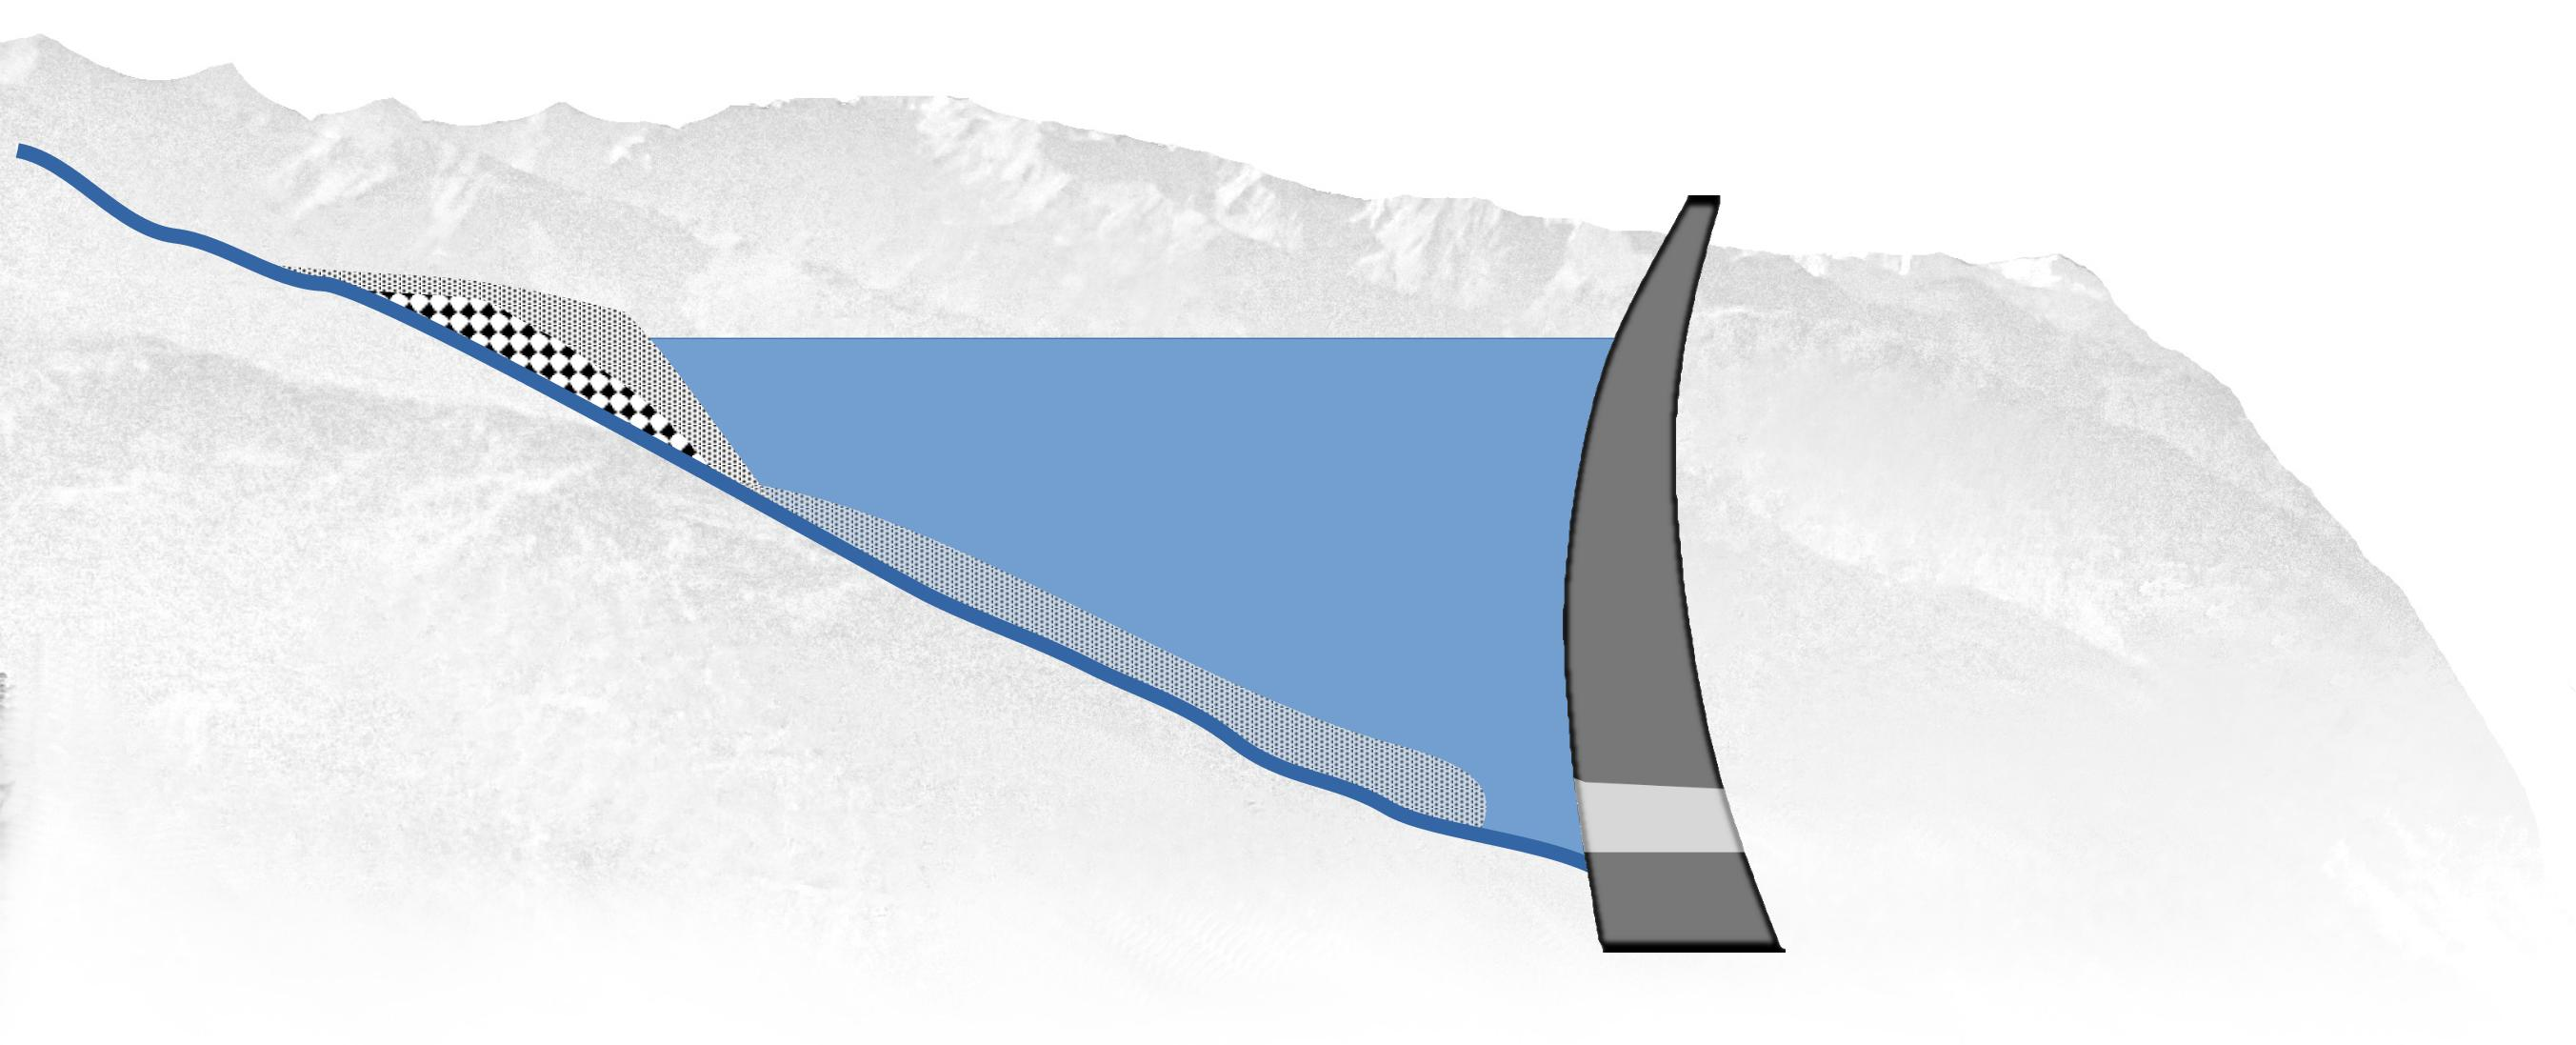
\includegraphics[width=0.91\paperwidth]{dam-scheme-zoom}};
		\end{scope}}
		\onslide<2->{
			\begin{scope}
				\node[anchor=south west, xshift=0.0\paperwidth, yshift=0.48\paperheight] {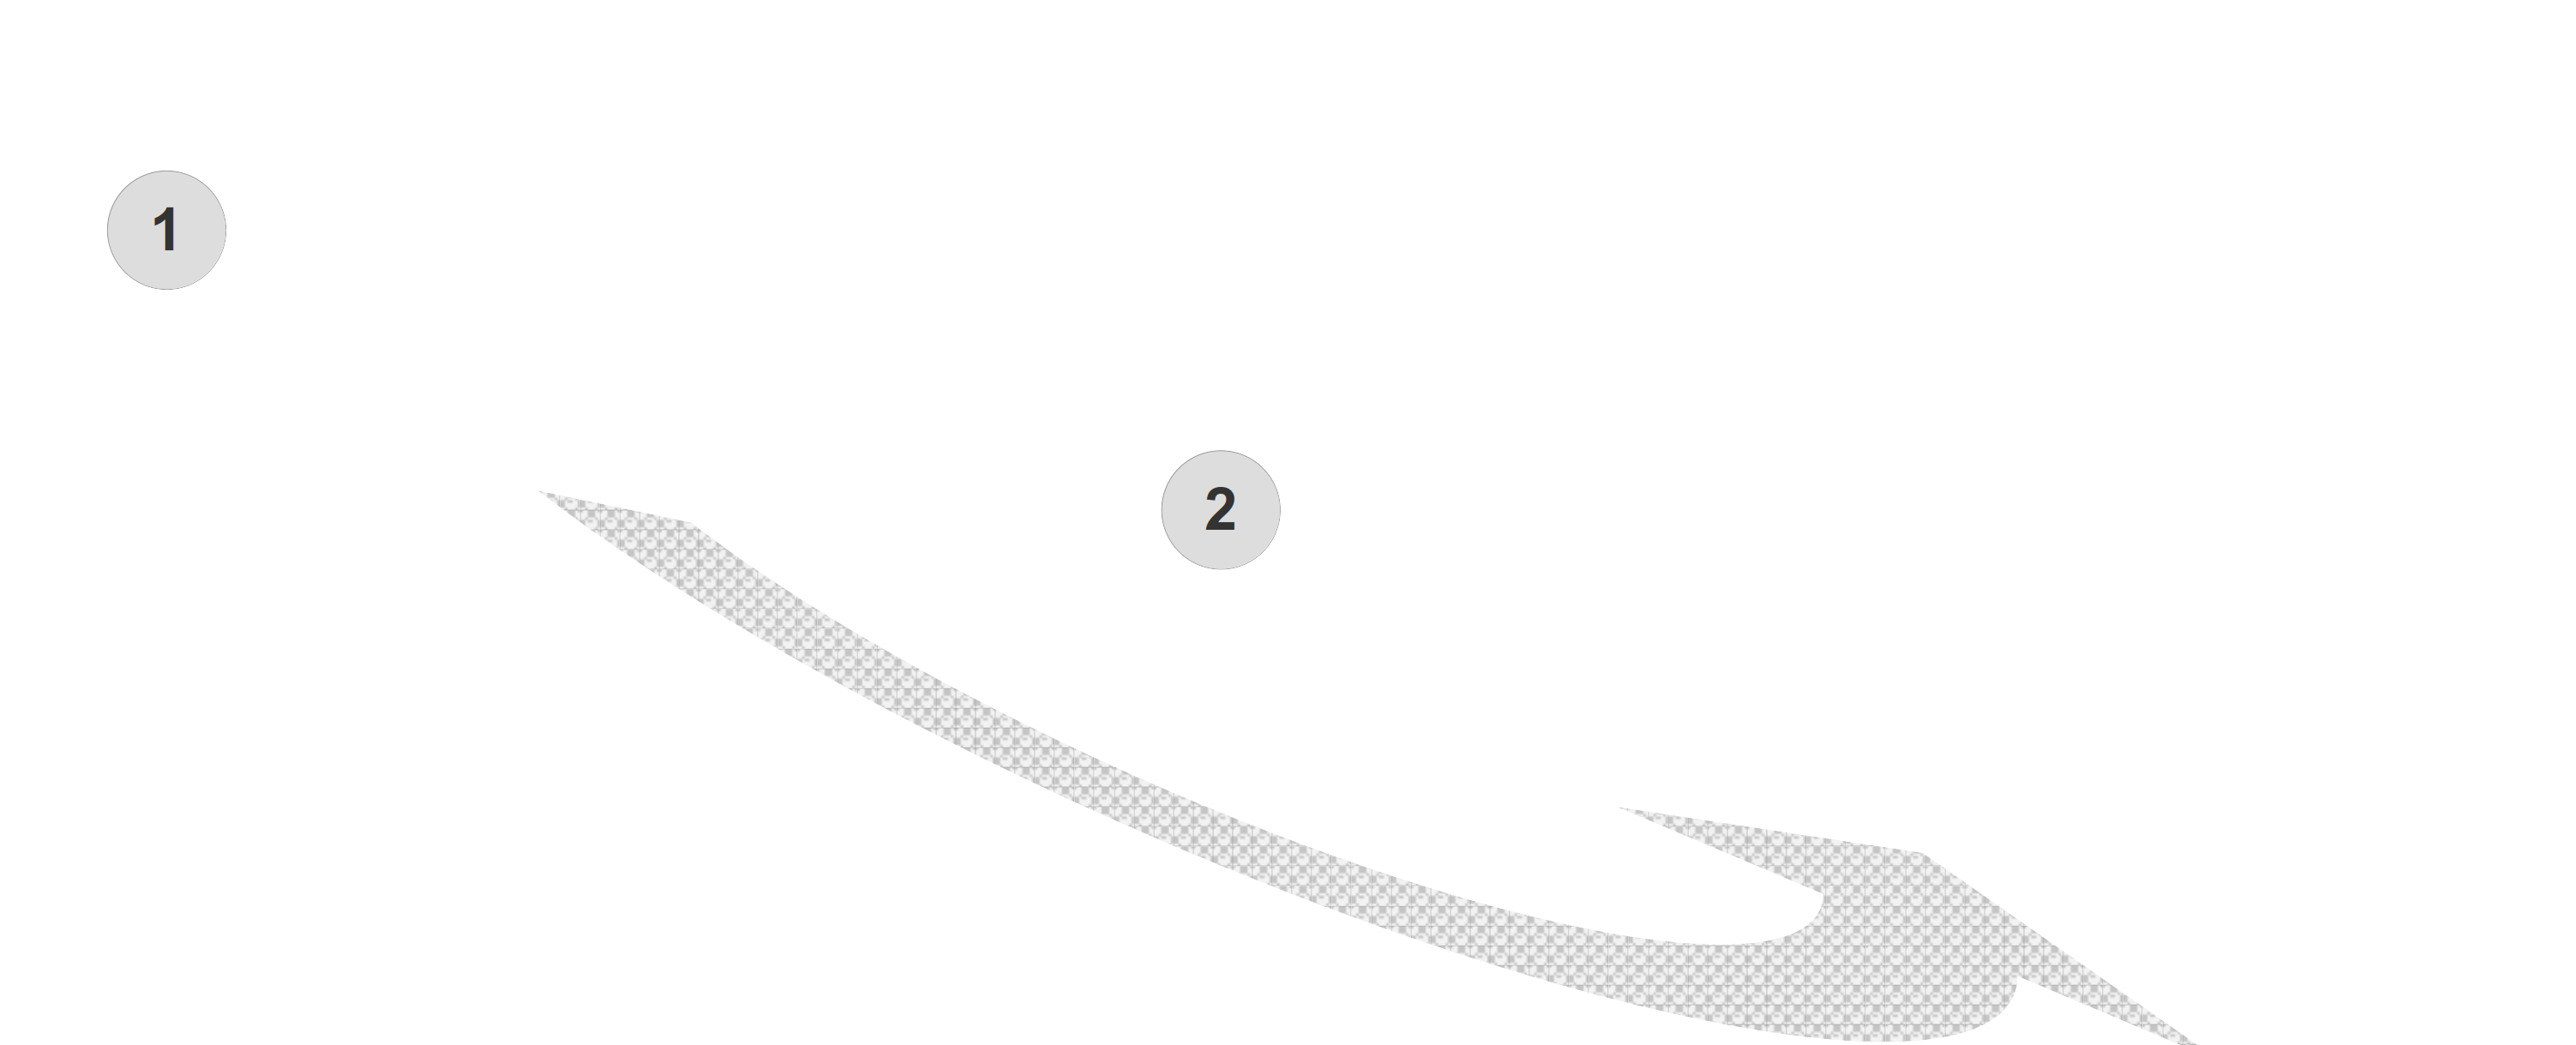
\includegraphics[width=0.91\paperwidth]{dam-scheme-zoom-overlay}};
		\end{scope}}
		\onslide<1->{
		\begin{scope}
			\node[anchor=south west, xshift=0.0\paperwidth, yshift=0.32\paperheight] {
			\begin{minipage}{0.95\textwidth}
				\begin{itemize}
					% \setlength\itemsep{0.7em}
					\item[\faHandORight]\ Coarse \& fine sediment deposits in delta regions (reservoir head)
					\item[\faHandORight]\ Very fine, partially cohesive sediment disperses in the entire reservoir
					\item[\faHandORight]\ Turbidity currents move suspended sediment close to dams
				\end{itemize}
			\end{minipage}
		};
		\end{scope}}
		\onslide<1->{
		\node[anchor=south west, xshift=0.33\paperwidth, yshift=2.1947cm, text=black, text width=0.5\paperwidth,align=left]{\tiny \textcolor{gray}{Image concept from Chamoun \textit{et al.} (2017) / SCCER-SoE}};}
	\end{tikzpicture}
\end{frame}

\subsection{Solution \raisebox{.5pt}{\textcircled{\raisebox{-.9pt} {1}}} Mountain River Training}
\begin{frame}{\secname\vspace{0.1cm}\\\textcolor{anthrazit!80!white}{\subsecname}}
	\begin{tikzpicture}
		\clip (0,0) rectangle (\paperwidth,\paperheight);
		\onslide<1->{
		\begin{scope}
				\node[anchor=south west, xshift=0.0\paperwidth, yshift=0.31\paperheight] {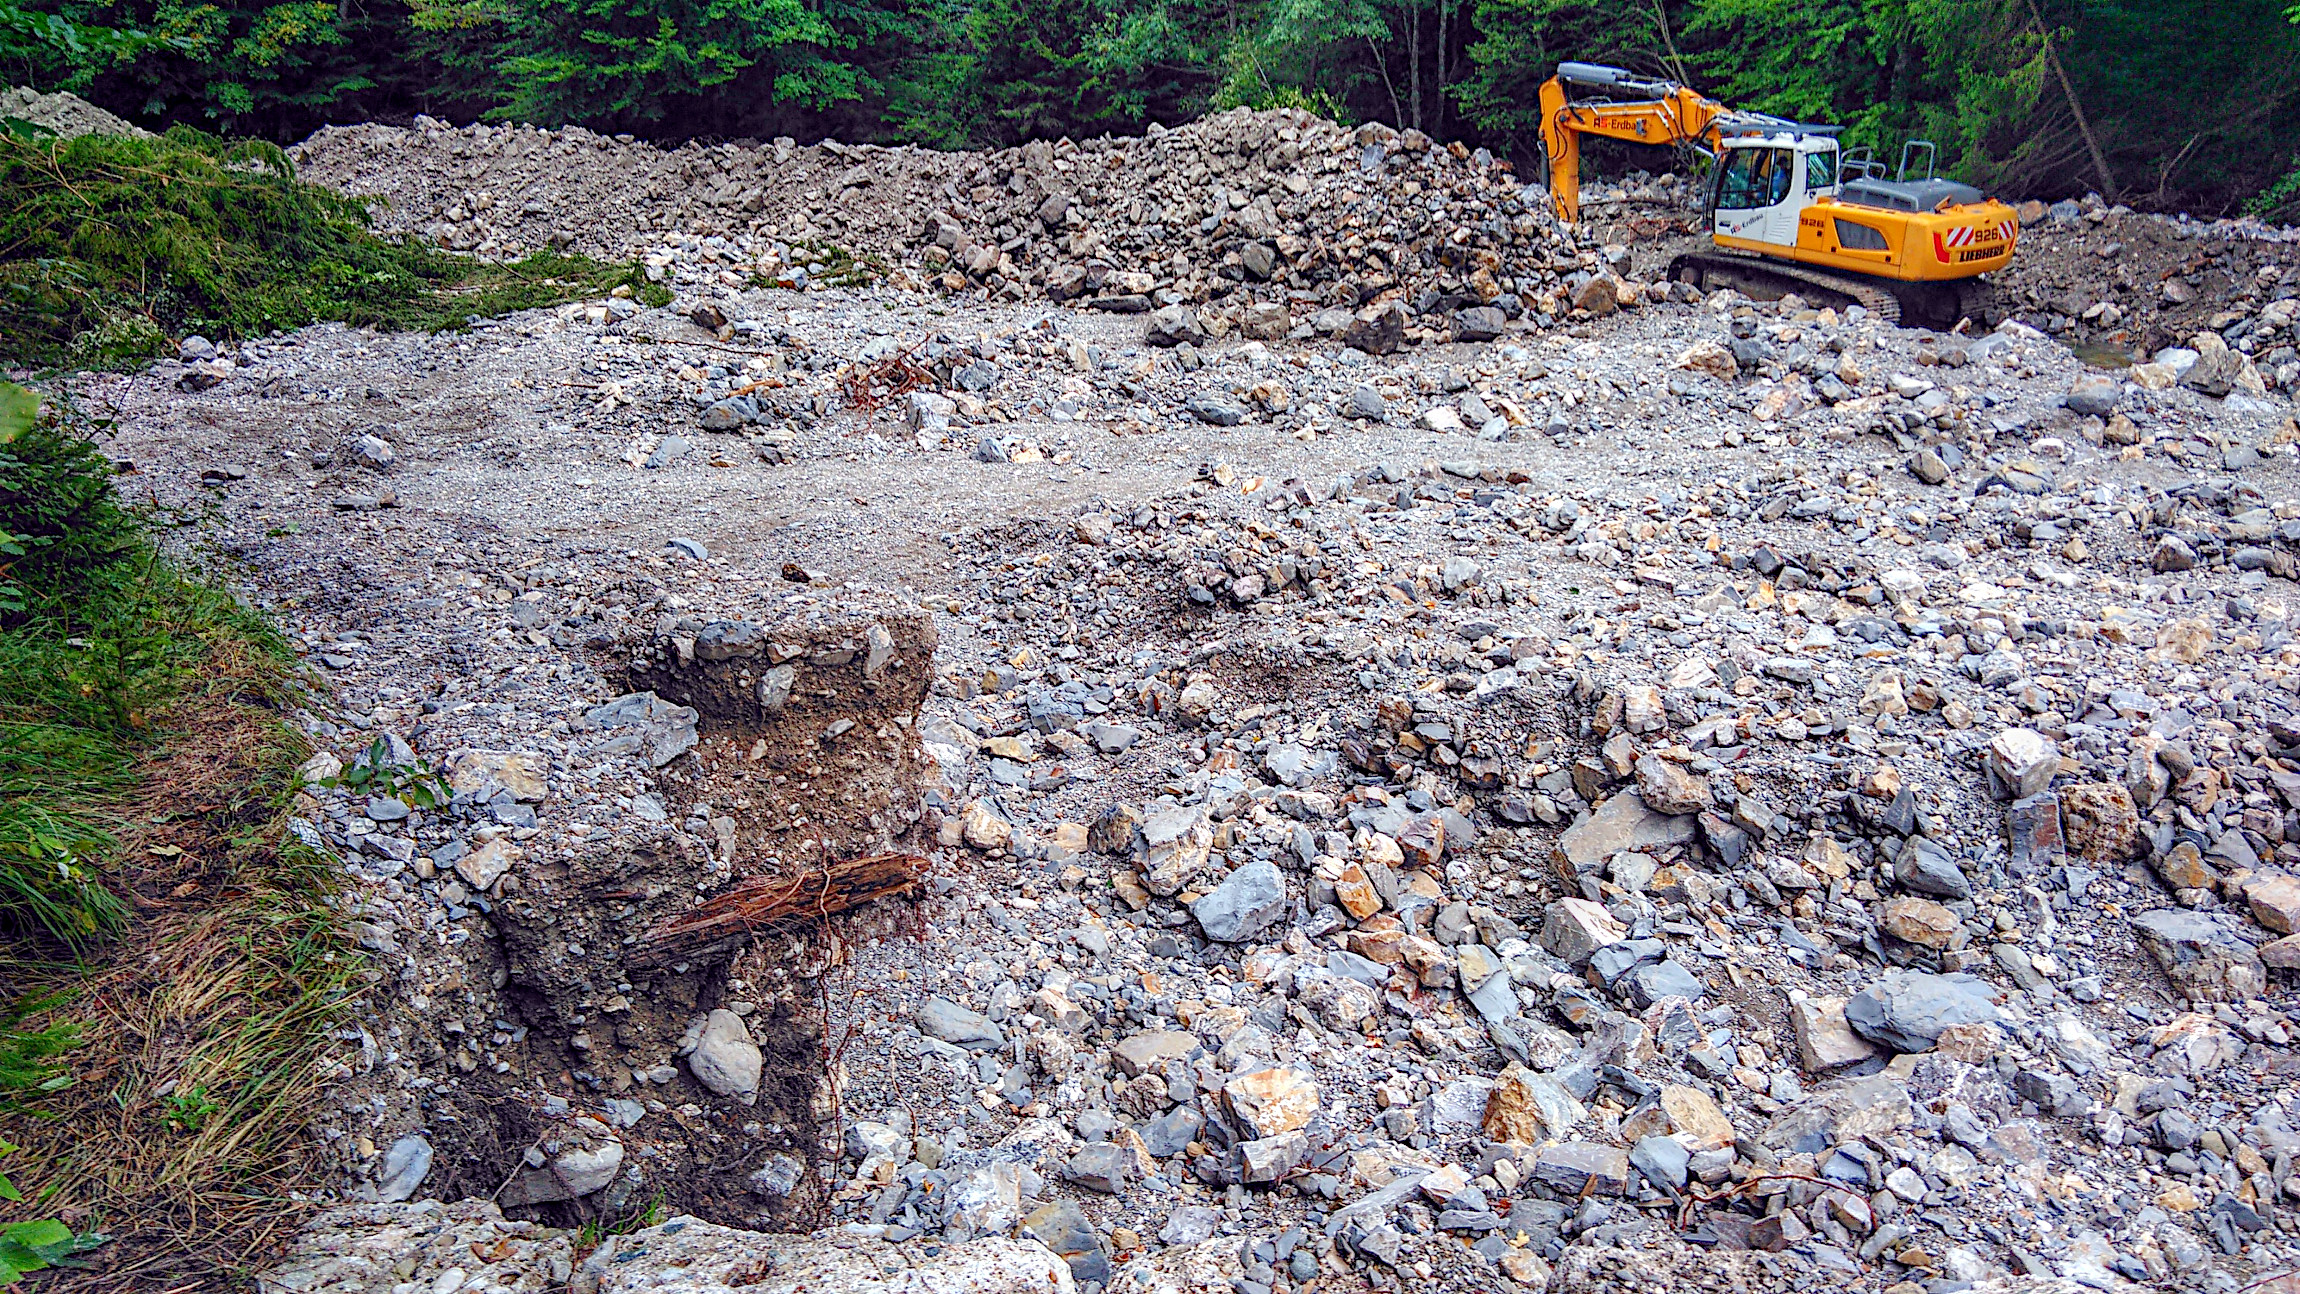
\includegraphics[width=0.865\paperwidth]{jenbach-bagger}};
		\end{scope}}
		\node[anchor=south west, xshift=0.33\paperwidth, yshift=2.13cm, text=black, text width=0.5\paperwidth,align=left]{\tiny \textcolor{gray}{Jenbach, Bavarian Alps}};
	\end{tikzpicture}
\end{frame}
\begin{frame}{\secname\vspace{0.1cm}\\\textcolor{anthrazit!80!white}{\subsecname}}
	\begin{tikzpicture}
		\clip (0,0) rectangle (\paperwidth,\paperheight);
		\onslide<1->{
			\begin{scope}
				\node[anchor=south west, xshift=0.0\paperwidth, yshift=0.31\paperheight] {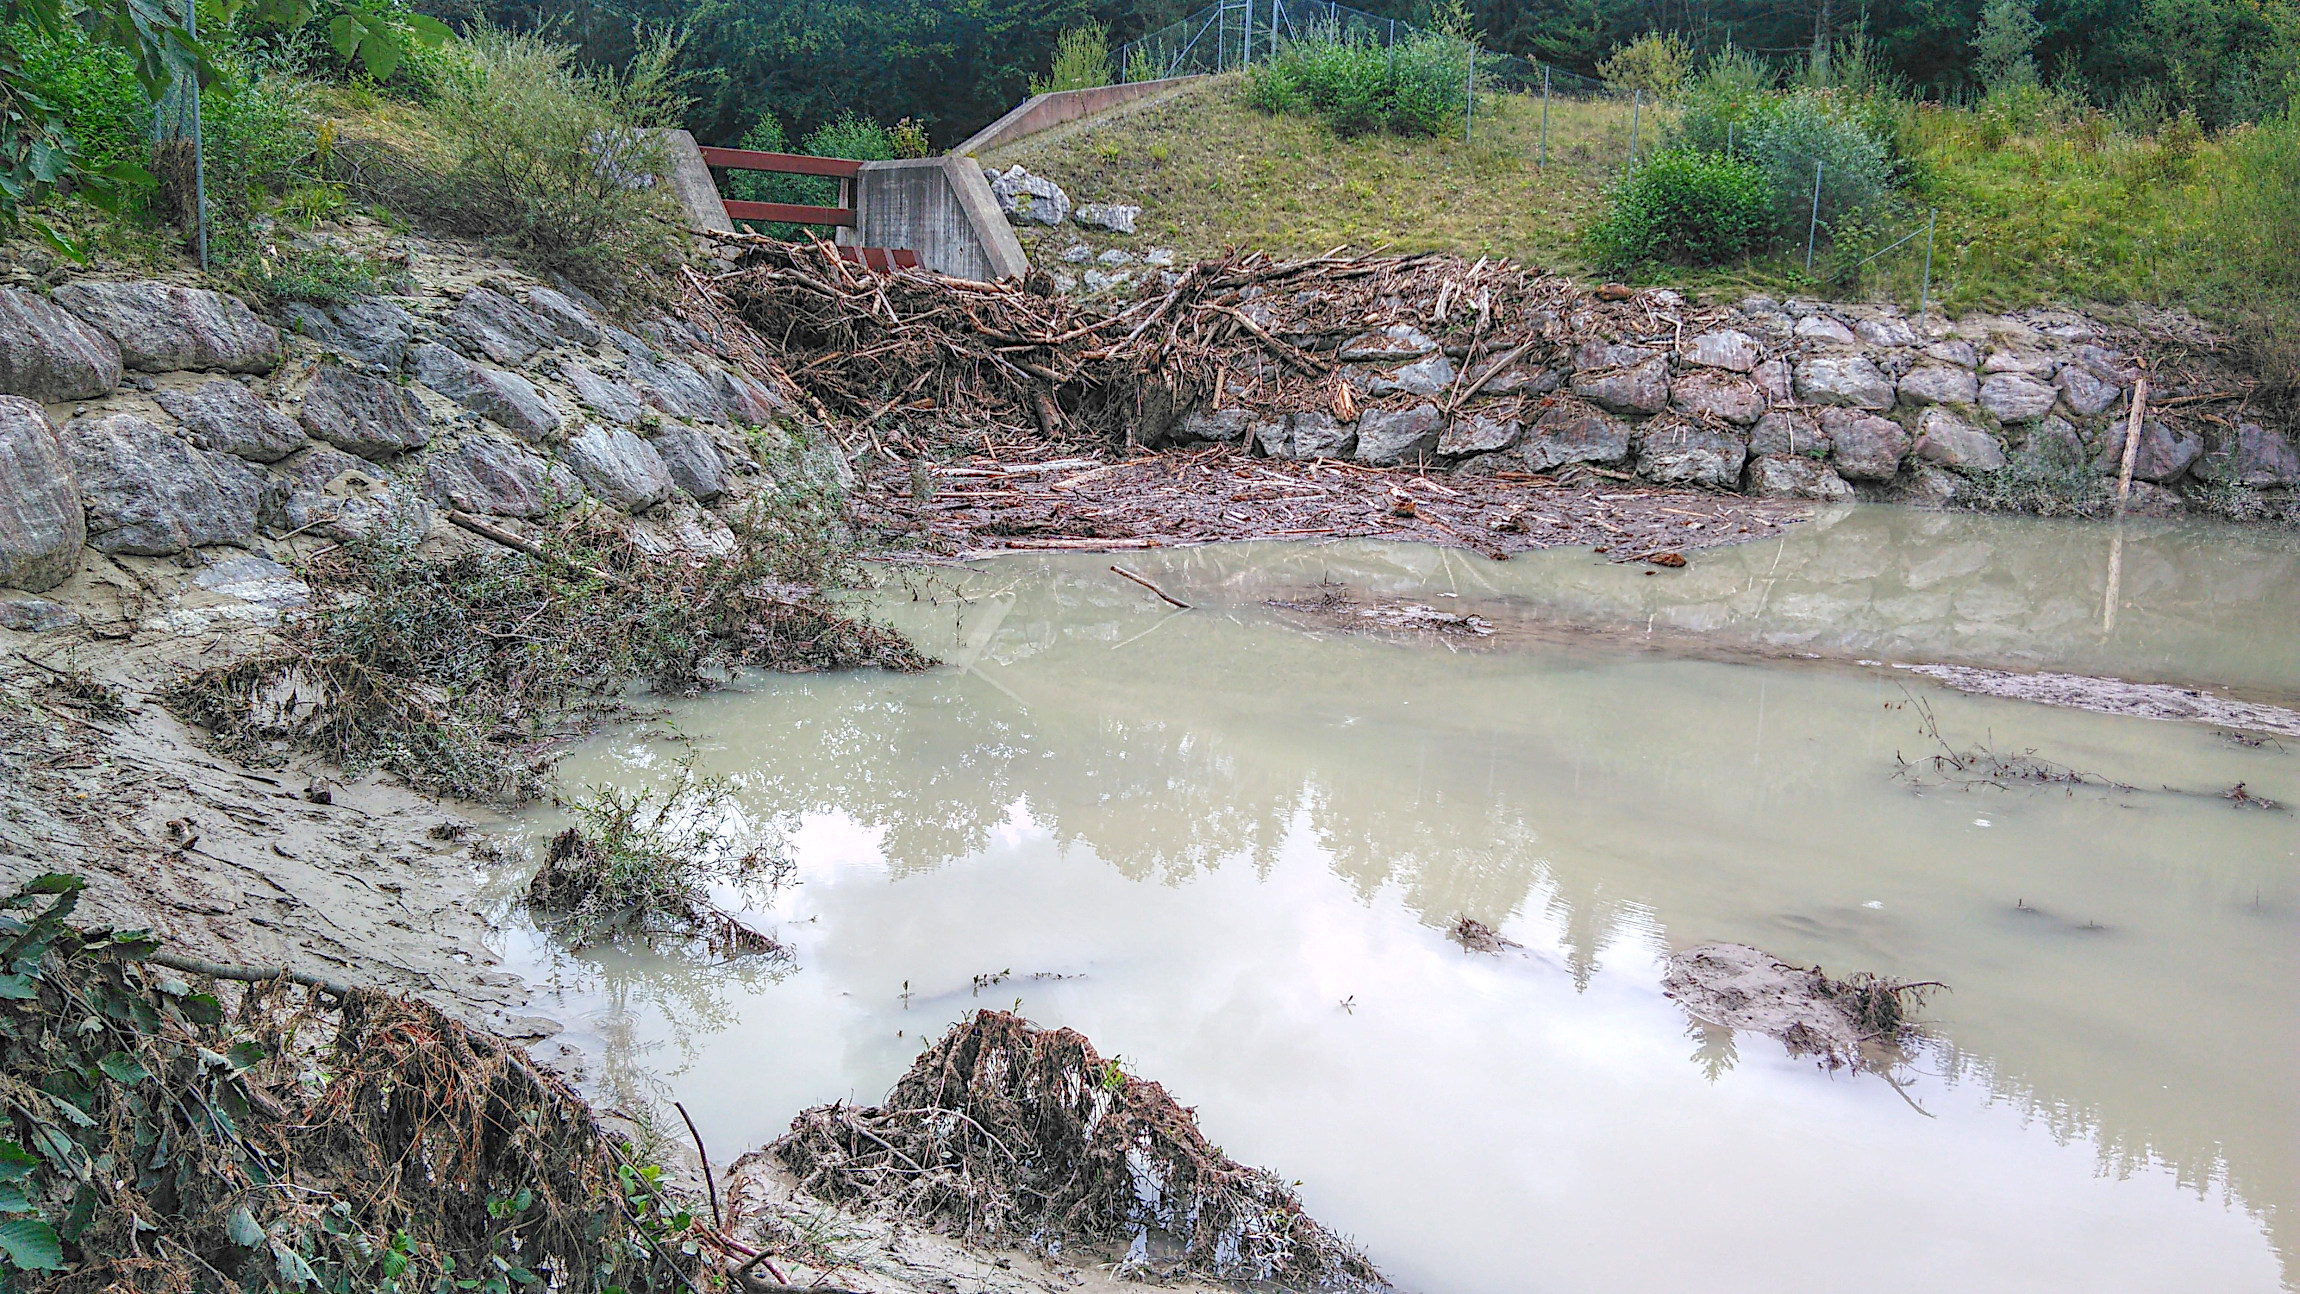
\includegraphics[width=0.865\paperwidth]{jenbach-trap-filled}};
		\end{scope}}
	\node[anchor=south west, xshift=0.33\paperwidth, yshift=2.13cm, text=black, text width=0.5\paperwidth,align=left]{\tiny \textcolor{gray}{Jenbach, Bavarian Alps}};
	\end{tikzpicture}
\end{frame}



\begin{frame}{\secname\vspace{0.1cm}\\\textcolor{anthrazit!80!white}{\subsecname}}
	\begin{tikzpicture}
		\clip (0,0) rectangle (\paperwidth,\paperheight);
		\onslide<1->{
			\begin{scope}
				\node[anchor=south west, xshift=0.0\paperwidth, yshift=0.34\paperheight] {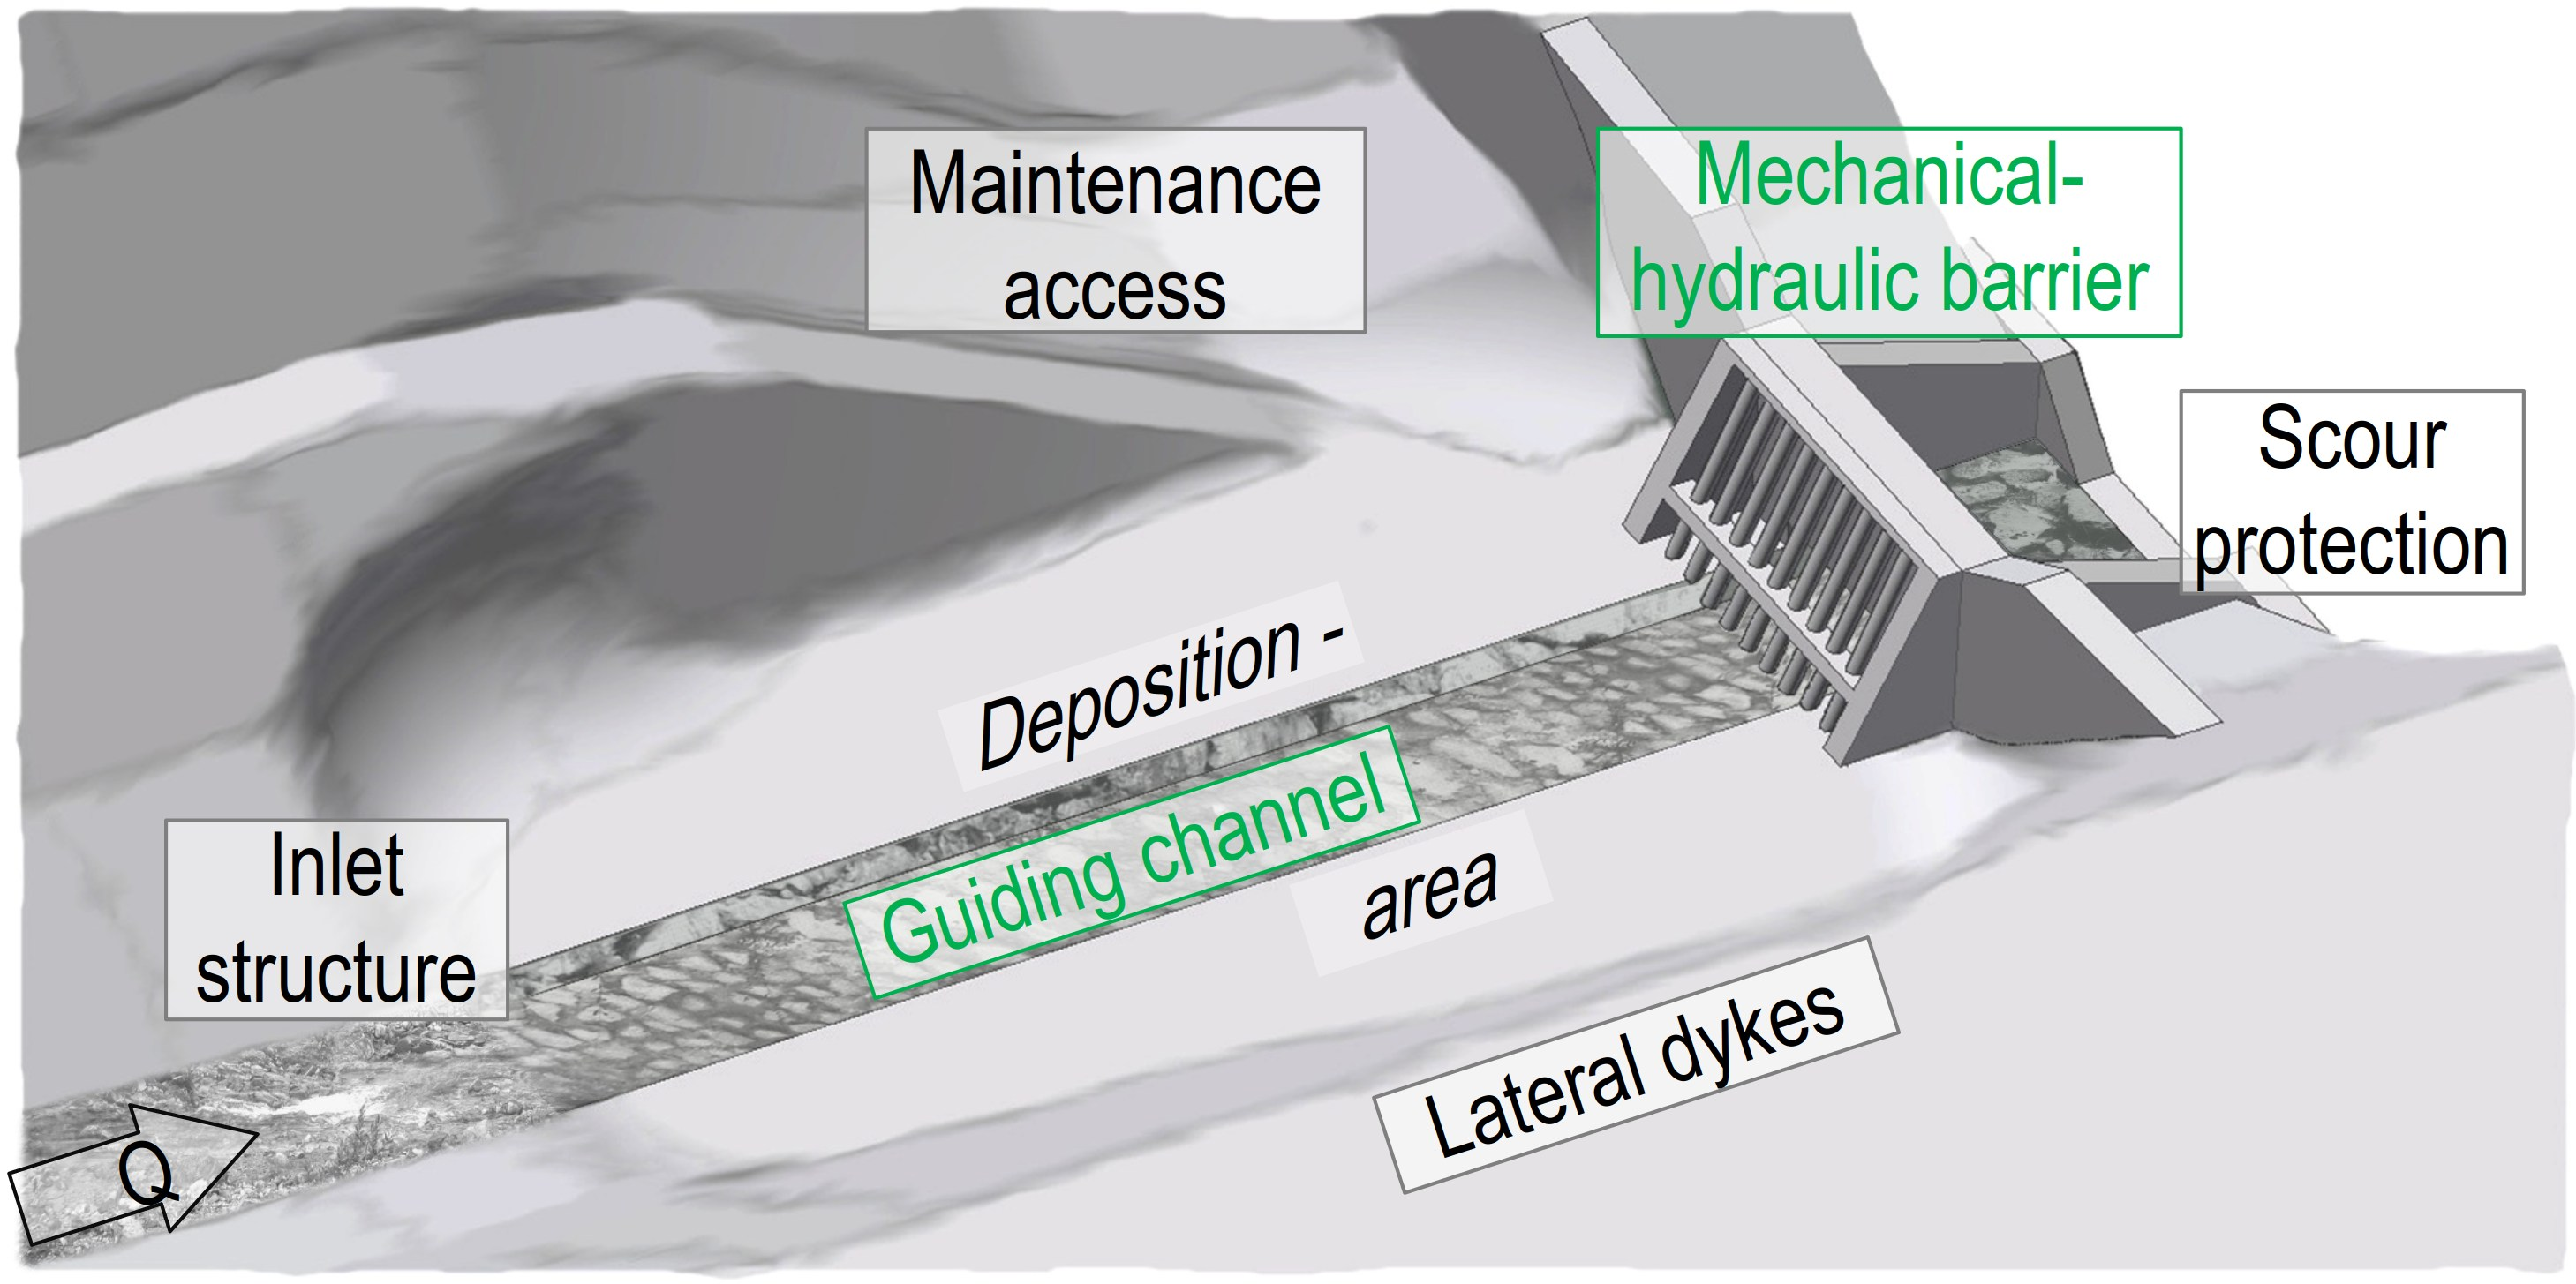
\includegraphics[width=0.88	\paperwidth]{check-dam-concept}};
		\end{scope}}
		\onslide<1-1>{
			\node[anchor=south west, xshift=0.33\paperwidth, yshift=2.13cm, text=black, text width=0.5\paperwidth,align=left]{\tiny \textcolor{gray}{Source: \sscURL{Schwindt \textit{et al.} (2018)}{https://www.nat-hazards-earth-syst-sci.net/18/647/2018/} / \sscURL{Moldenhauer, Piton, Schwindt \textit{et al.}}{https://www.sciencedirect.com/science/article/pii/S1001627920300792}}};}
	\end{tikzpicture}
\end{frame}

\subsection{Solution \raisebox{.5pt}{\textcircled{\raisebox{-.9pt} {2}}} Manage Sediment in Reservoirs}
\begin{frame}{\secname\vspace{0.1cm}\\\textcolor{anthrazit!80!white}{\subsecname}}
	\begin{tikzpicture}
		\clip (0,0) rectangle (\paperwidth,\paperheight);
		\onslide<1->{
		\begin{scope}
			\node[anchor=south west, xshift=0.05\paperwidth, yshift=0.4\paperheight] {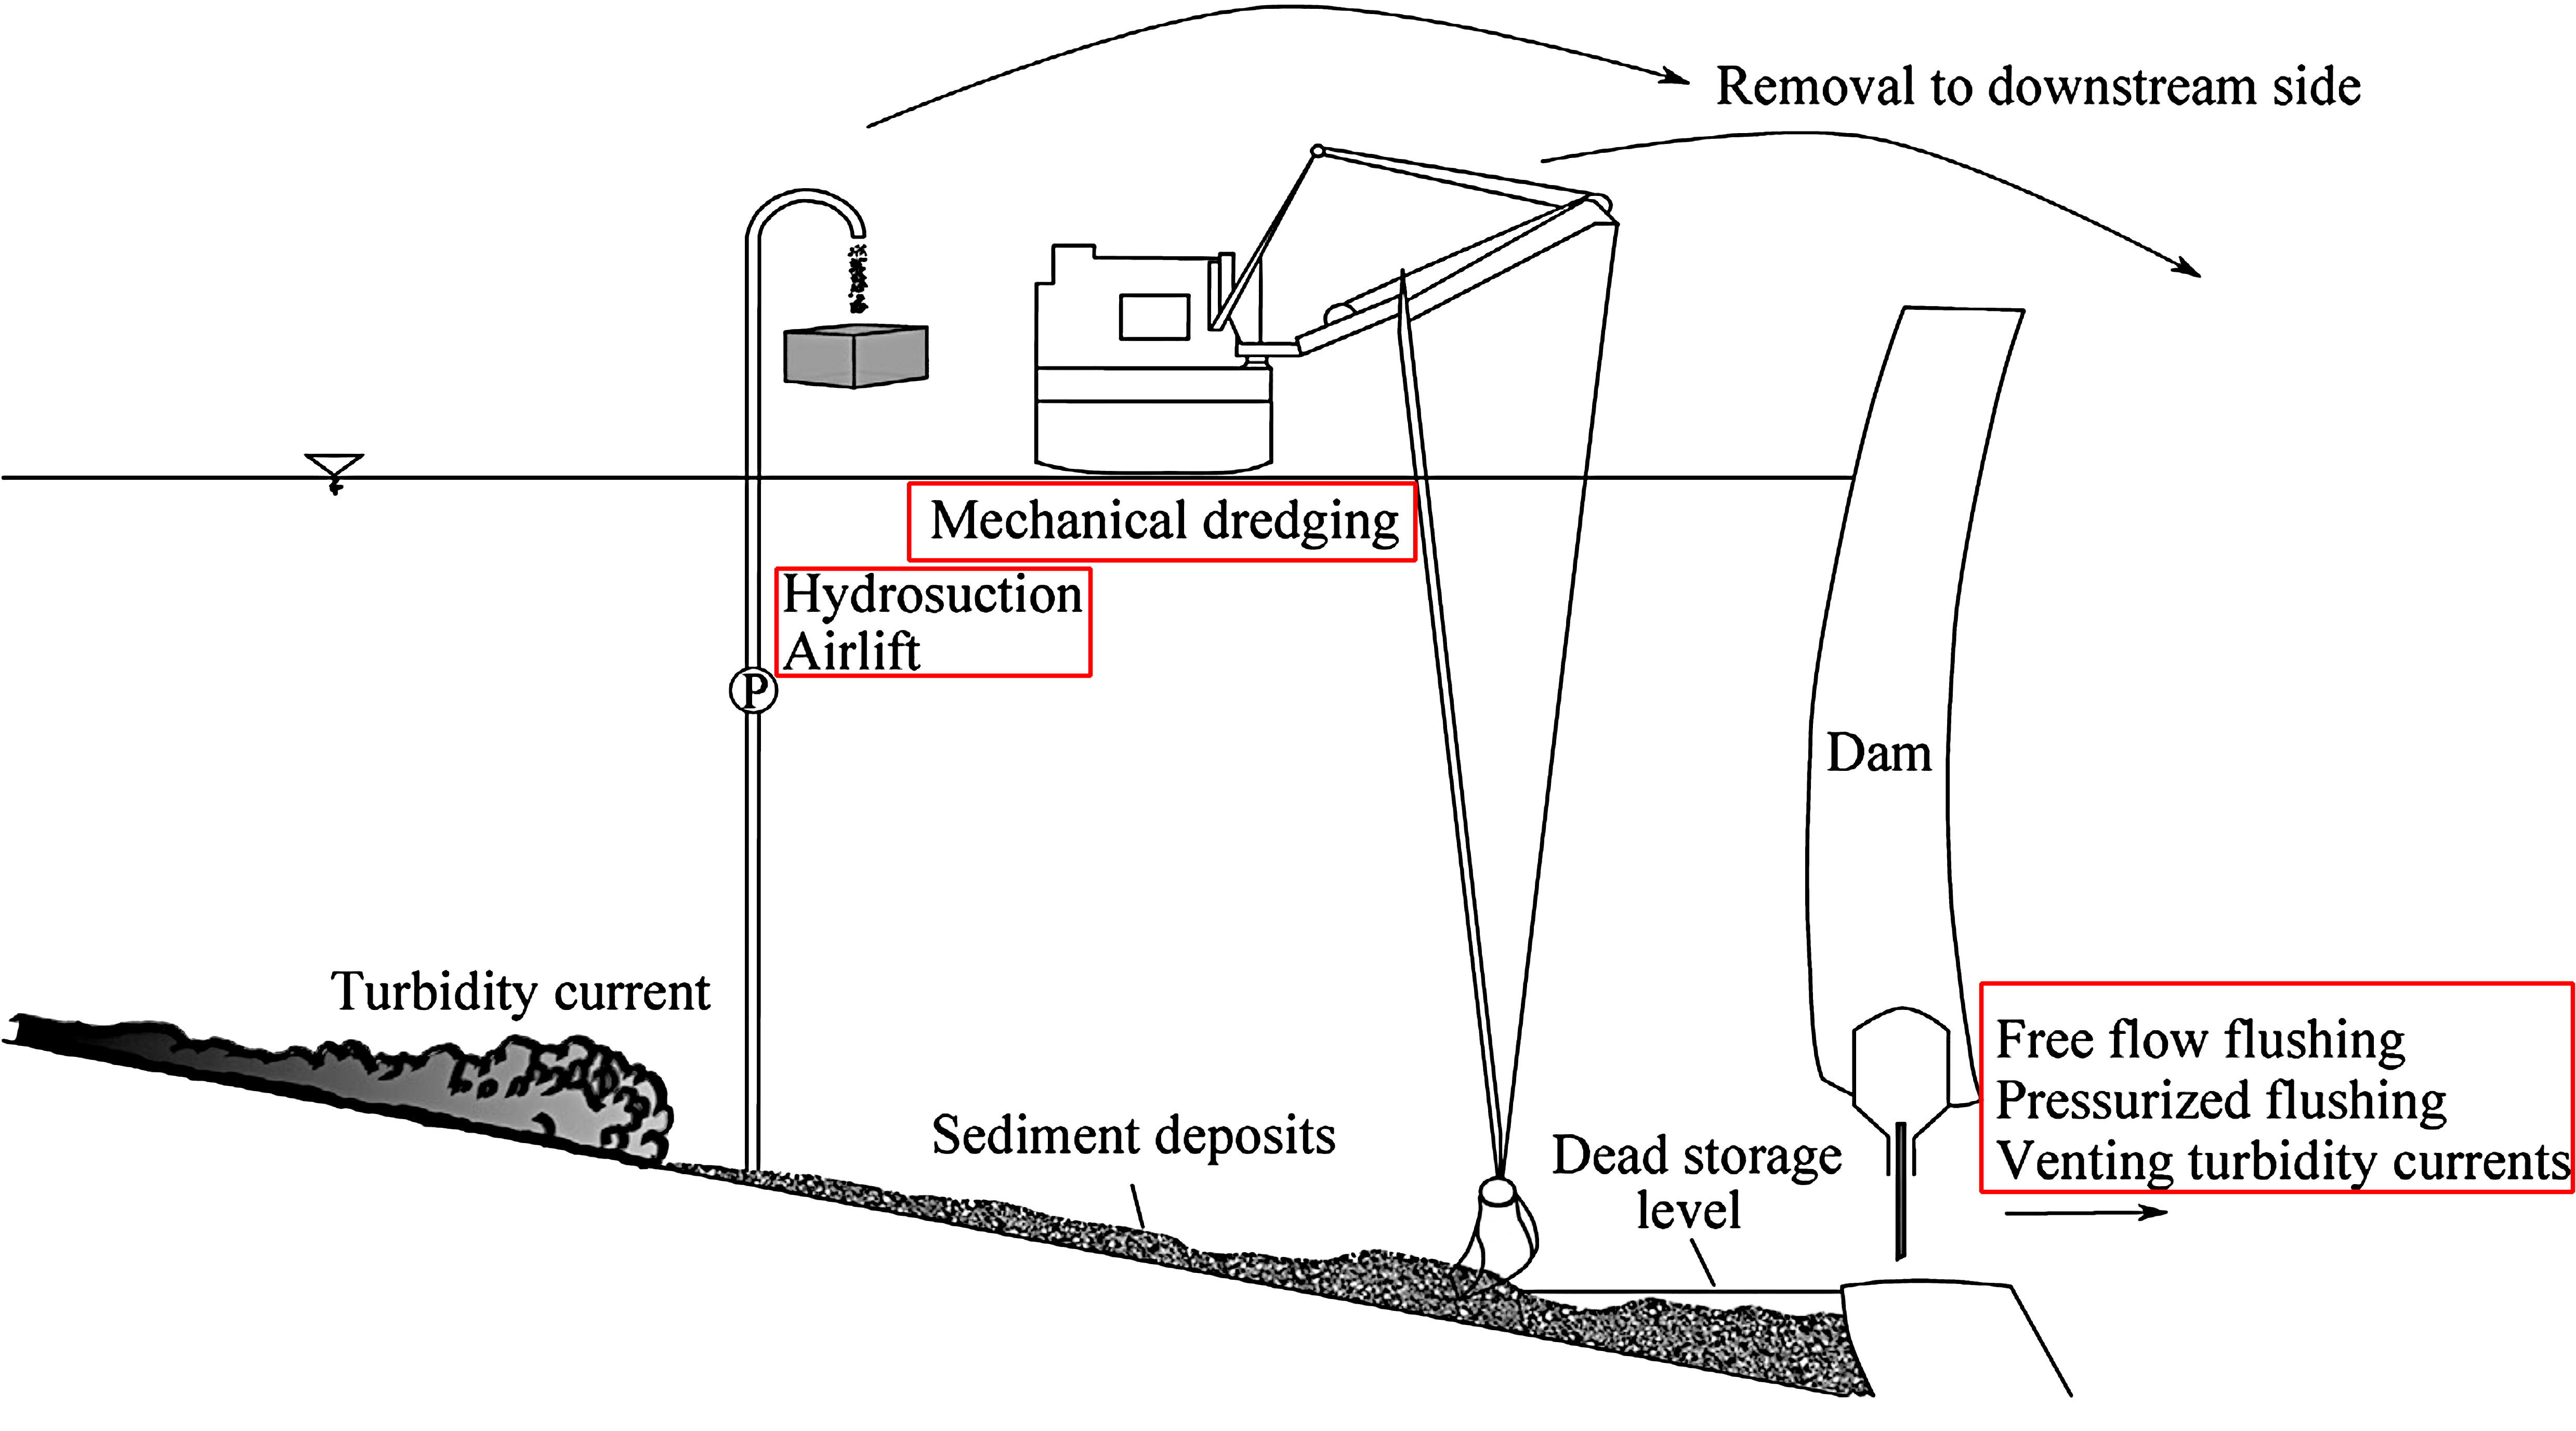
\includegraphics[width=0.78	\paperwidth]{reservoir-sedimentation-mgmt-highlight}};
		\end{scope}}
		\onslide<1->{
		\begin{scope}
			\node[anchor=south west, xshift=0.0\paperwidth, yshift=0.3\paperheight] {
				\begin{minipage}{0.95\textwidth}
					\begin{itemize}
						\item[\faHandORight]\ Airlift / hydrosuction
						\item[\faHandORight]\ Mechanical dredging
						\item[\faHandORight]\ Flushing (free flow, pressurized, venting) \& re-suspension
						\item[\faHandORight]\ Sediment bypass tunnels
					\end{itemize}
				\end{minipage}
			};
		\end{scope}}
		\onslide<1-1>{
			\node[anchor=south west, xshift=0.33\paperwidth, yshift=2.13cm, text=black, text width=0.5\paperwidth,align=left]{\tiny \textcolor{gray}{Source: Chamoun \textit{et al.} / SCCER-SoE (2018)}};}
	\end{tikzpicture}
\end{frame}


%\subsection{Sediment Continuity - Measuring \& Modeling}
\begin{frame}{\secname\vspace{0.1cm}\\\textcolor{anthrazit!80!white}{\subsecname}}
	\begin{tikzpicture}
		\clip (0,0) rectangle (\paperwidth,\paperheight);
		\onslide<1->{
		\begin{scope}
			\node[anchor=south west, xshift=0.0\paperwidth, yshift=0.3\paperheight] {
			\begin{minipage}{0.9999\textwidth}
			\begin{tcolorbox}[colbacktitle=unisblue!60!black, colback=unisblue!20!white, fonttitle=\bfseries, standard jigsaw,colframe=unisblue, bottom=0mm, middle=0mm, boxsep=0.2mm, opacityframe=0.5, opacityfill=0.7, opacitybacktitle=0.95, title filled, title={Planning sediment management in reservoirs}, size=fbox]
				\vspace{0.25cm}		 
				\begin{itemize}			
					\item[\faCog] Engineering solutions to bypass coarse sediment...
					\begin{itemize}
						\item[...] are  very expensive
						\item[...] require case-specific optimization: \textbf{field, laboratory, or numerically}
					\end{itemize}
					\onslide<2->{
					\item[\faCog] \textbf{Numerical modeling}...
					\begin{itemize}
						\item[...] virtually assesses management strategies \& mechanical interventions
						\item[...] is \textbf{cheaper} than field and laboratory tests
						\item[...] often is \textbf{imprecise} because of rigorous simplification of physical processes
					\end{itemize}}
					\onslide<4->{
					\item[\faCog] \textbf{Numerical model calibration} is difficult:
					\begin{itemize}
						\item[1.]  a reservoir model has \textbf{$n \geq$~3 calibration parameters} with unknown distributions \\$\rightarrow$ $n$-dimensional response surface with unknown shape
						\item[2.] \textbf{one model run takes $\mathcal{O}$ multiple days-weeks} to evaluate one calibration parameter combination
						\vspace{0.25cm}
					\end{itemize}
					\item[\faHandORight]\ \textbf{Surrogate-assisted Bayesian calibration}
					}
				\end{itemize}%\smallskip
			\end{tcolorbox}
			\end{minipage}
			};
		\end{scope}}
		\onslide<3-3>{
		\begin{scope}
			\node[opacity=0.8, anchor=south west, xshift=0.\paperwidth, yshift=0.1\paperheight] {
\includegraphics[width=\paperwidth]{white}};
		\end{scope}
		\begin{scope}
			\node[anchor=south west, xshift=0.1\paperwidth, yshift=0.41\paperheight] {
			\begin{minipage}{0.8\textwidth}
				\begin{tcolorbox}[colbacktitle=gray!80!black, colback=gray!40!white, fonttitle=\bfseries, standard jigsaw,colframe=gray, bottom=0mm, middle=0mm, boxsep=0.2mm, opacityframe=0.5, opacityfill=1.0, opacitybacktitle=0.95, title filled, title={\centering\faLightbulbO\ Calibration}, size=fbox]
					\vspace{0.25cm}
					{\hspace{4cm} \Huge \faRefresh }
%					\begin{itemize}
%						\item[\faHandORight] \textbf{Calibration} is an inverse, multi-step problem to reduce model uncertainty to achieve good agreement between modeled and measured data with reasonable tolerance.
%						\item[\faHandORight] \textbf{Iterative} process: fit (bulk) model parameters within a physically reasonable range, update the model, and compare observations with model results.
%					\end{itemize}\smallskip
%					\par {\tiny\hfill \textcolor{gray!80!black}{Sources: Oberkampf \textit{et al.} (2004), Wright \textit{et al.} (2017), Schwindt \textit{et al.} (2023)}}
				\end{tcolorbox}\smallskip
			\end{minipage}};
		\end{scope}}
	\end{tikzpicture}
\end{frame}

\subsection{Surrogate-Assisted Bayesian Calibration of Numerical Models}

\begin{frame}{\secname\vspace{0.1cm}\\\textcolor{anthrazit!80!white}{\subsecname}}
	\begin{tikzpicture}
		\clip (0,0) rectangle (\paperwidth,\paperheight);
		\onslide<2->{
		\begin{scope}
			\node[anchor=south west, xshift=0.05\paperwidth, yshift=0.26\paperheight] {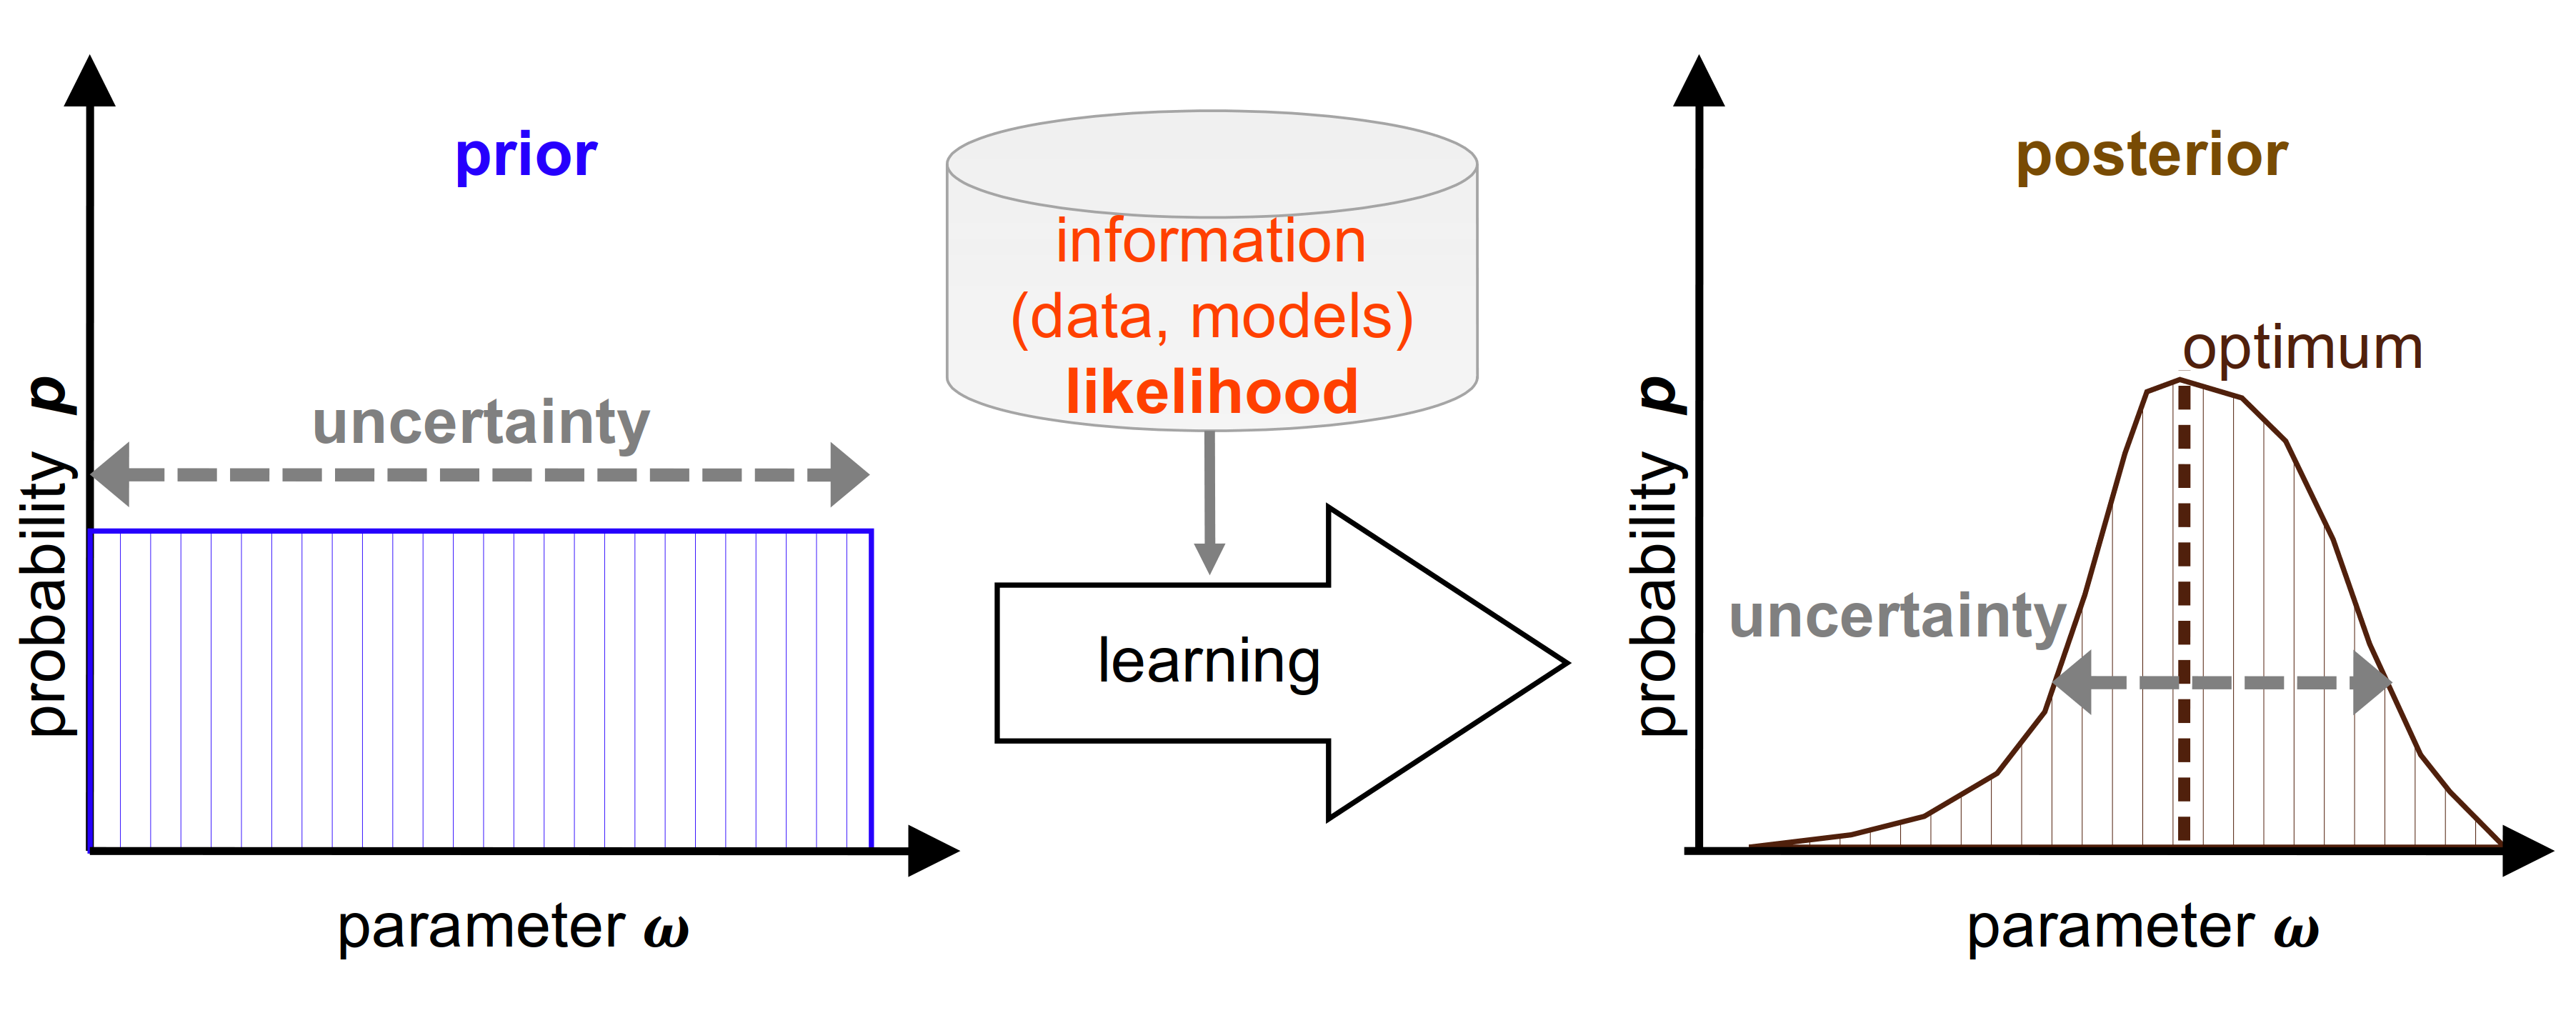
\includegraphics[width=0.78	\paperwidth]{caliBayes}};
		\end{scope}}
		\onslide<1->{
		\begin{scope}
			\node[anchor=south west, xshift=0cm, yshift=0.72\paperheight] {
				\begin{minipage}{\textwidth}
					\begin{center}			
						\textcolor{gray}{\textbf{Bayes' theorem}}\vspace{0.2cm}\\$\textcolor{brown}{\overbrace{p\left(\omega \mid \mathcal{M} \right)}^{posterior}} = \frac{\textcolor{orange!65!red}{\overbrace{p\left(\mathcal{M} \mid  \omega\right)}^{likelihood}} \cdot \textcolor{unisblue}{\overbrace{p\left(\omega\right)}^{prior}}}{\textcolor{black}{\underbrace{p\left(\mathcal{M} \right)}_{normalization}}}$
						% $p\left(\mathcal{M} \right)$~:=~normalization or Bayesian model evidence (\textit{here: constant})
					\end{center}
			\end{minipage}};
	\end{scope}}		
	\end{tikzpicture}
\end{frame}


\begin{frame}{\secname\vspace{0.1cm}\\\textcolor{anthrazit!80!white}{\subsecname}}
	\begin{tikzpicture}
		\clip (0,0) rectangle (\paperwidth,\paperheight);
		\onslide<1->{
		\begin{scope}
				\node[anchor=south west, xshift=0.0\paperwidth, yshift=0.27\paperheight] {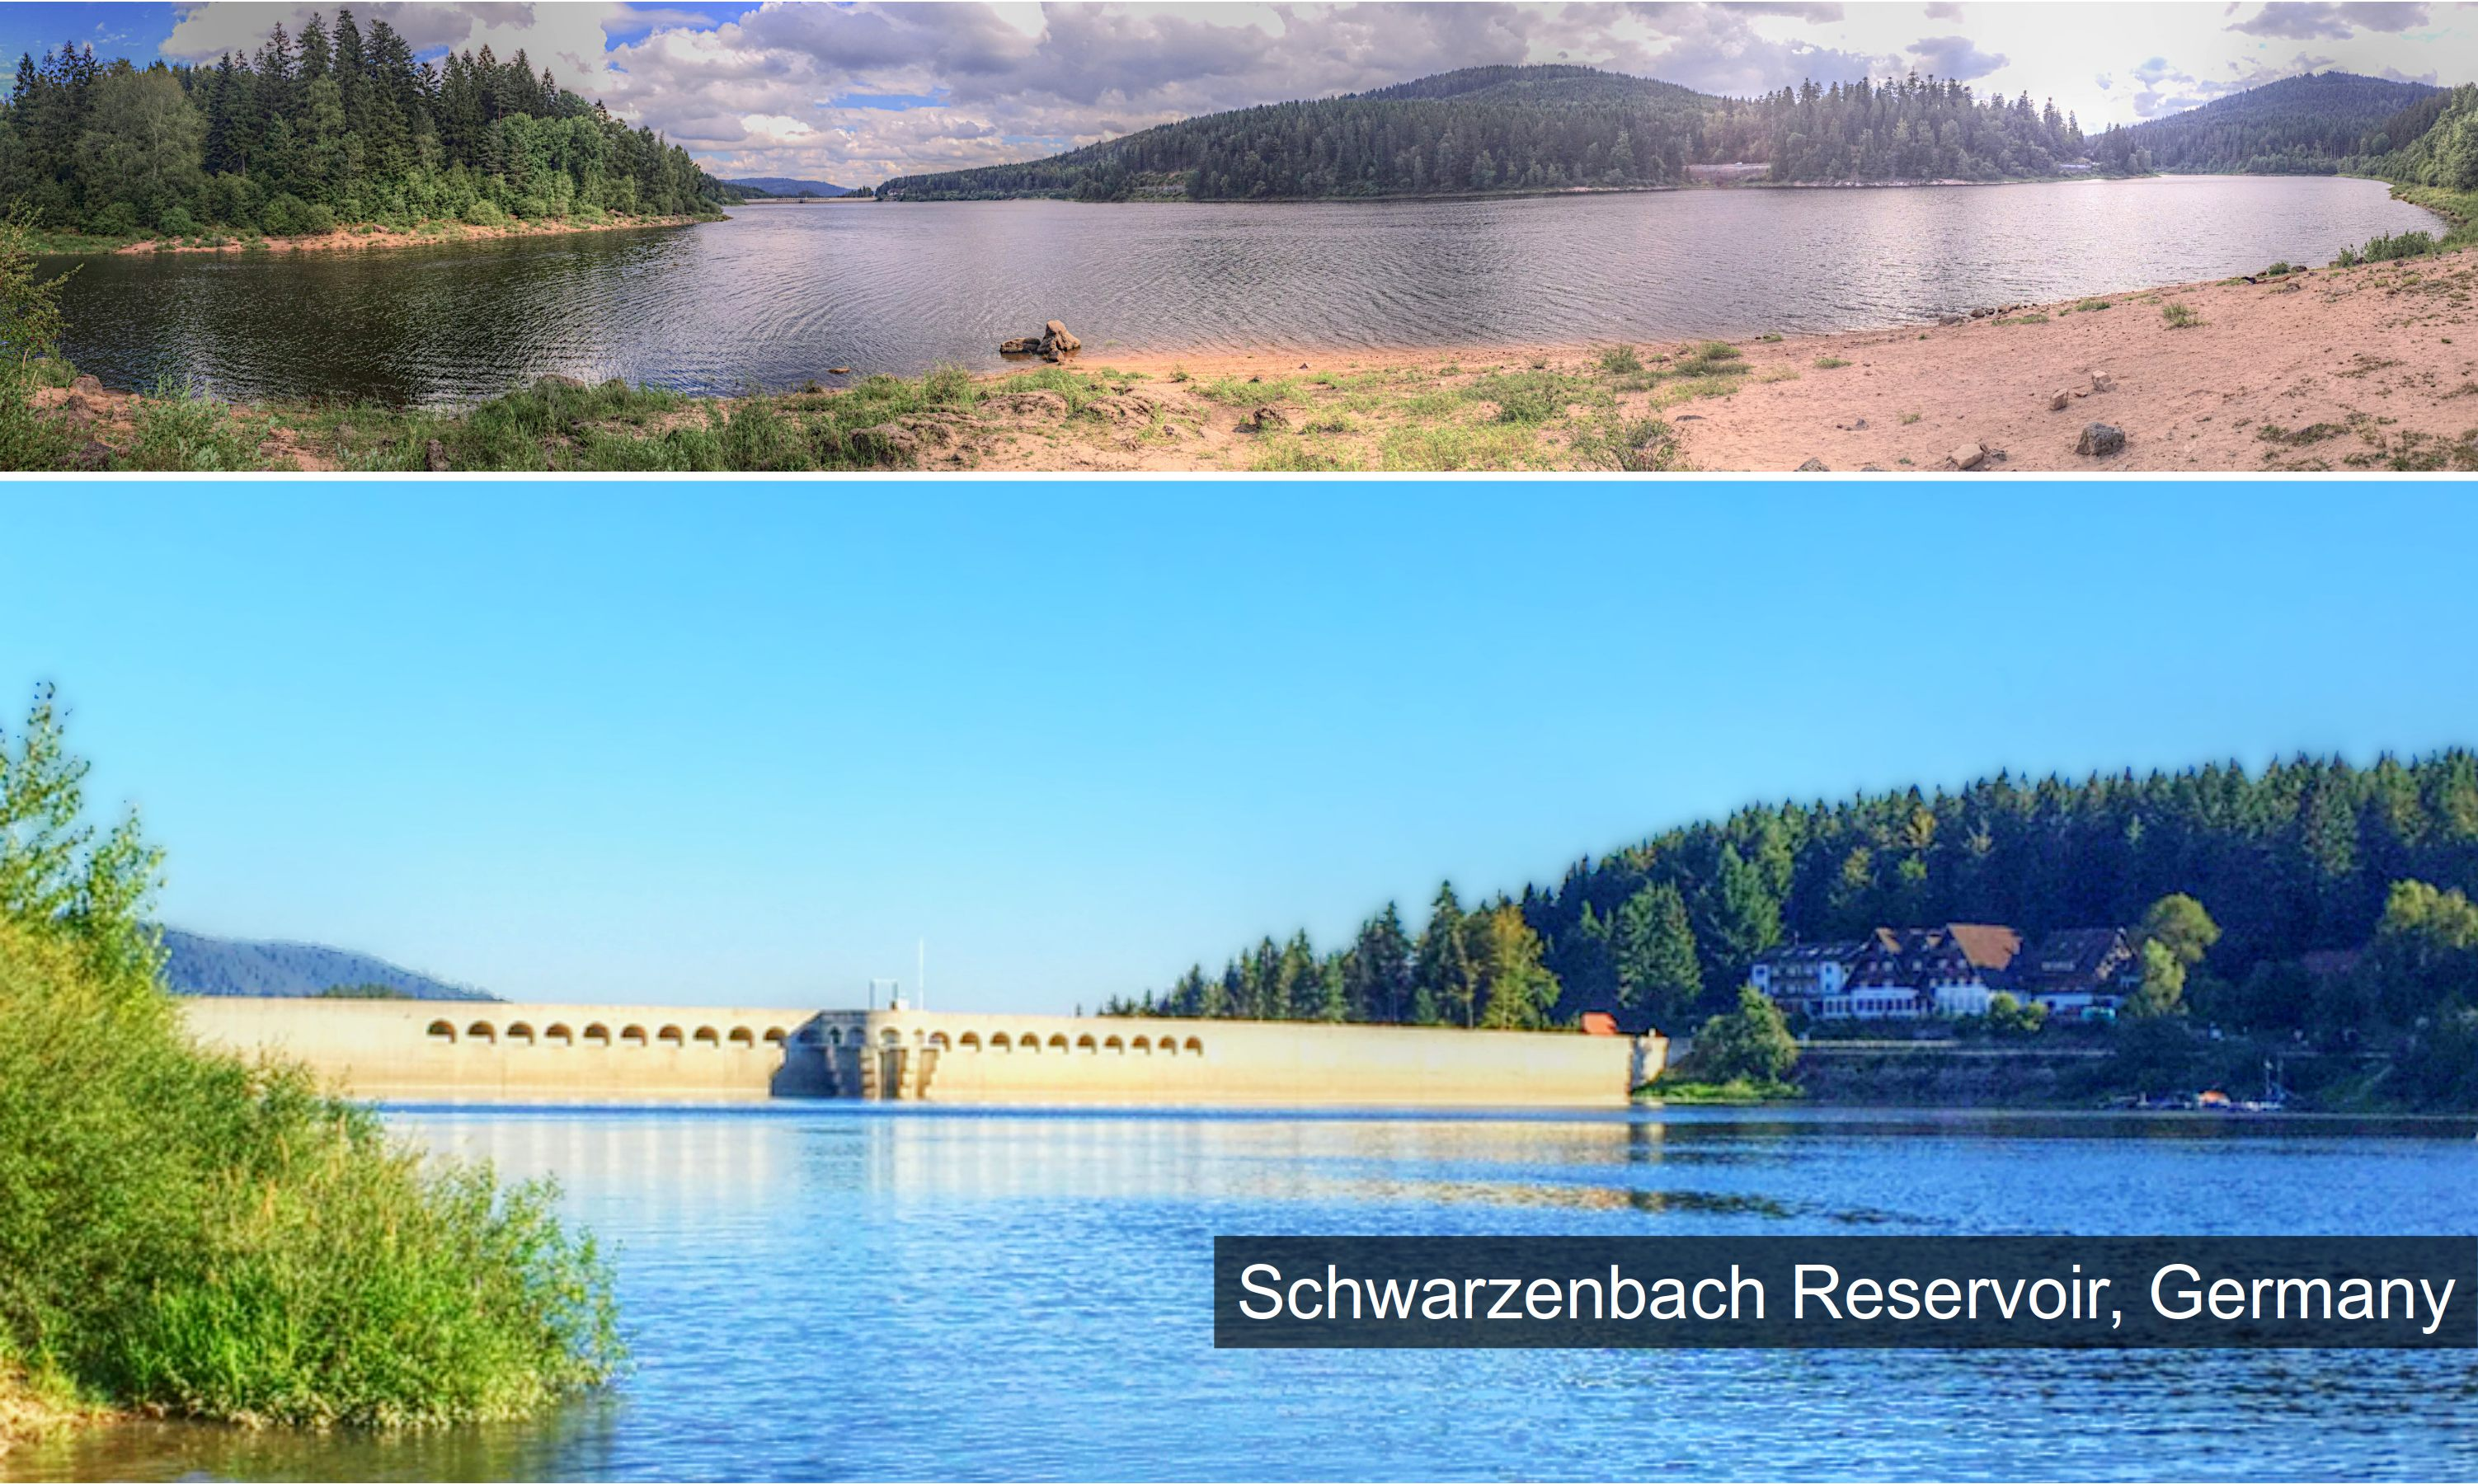
\includegraphics[width=0.88\paperwidth]{sbt-img}};
		\end{scope}}
		\onslide<2->{
			\begin{scope}
				\node[anchor=south west, xshift=0.0\paperwidth, yshift=0.27\paperheight] {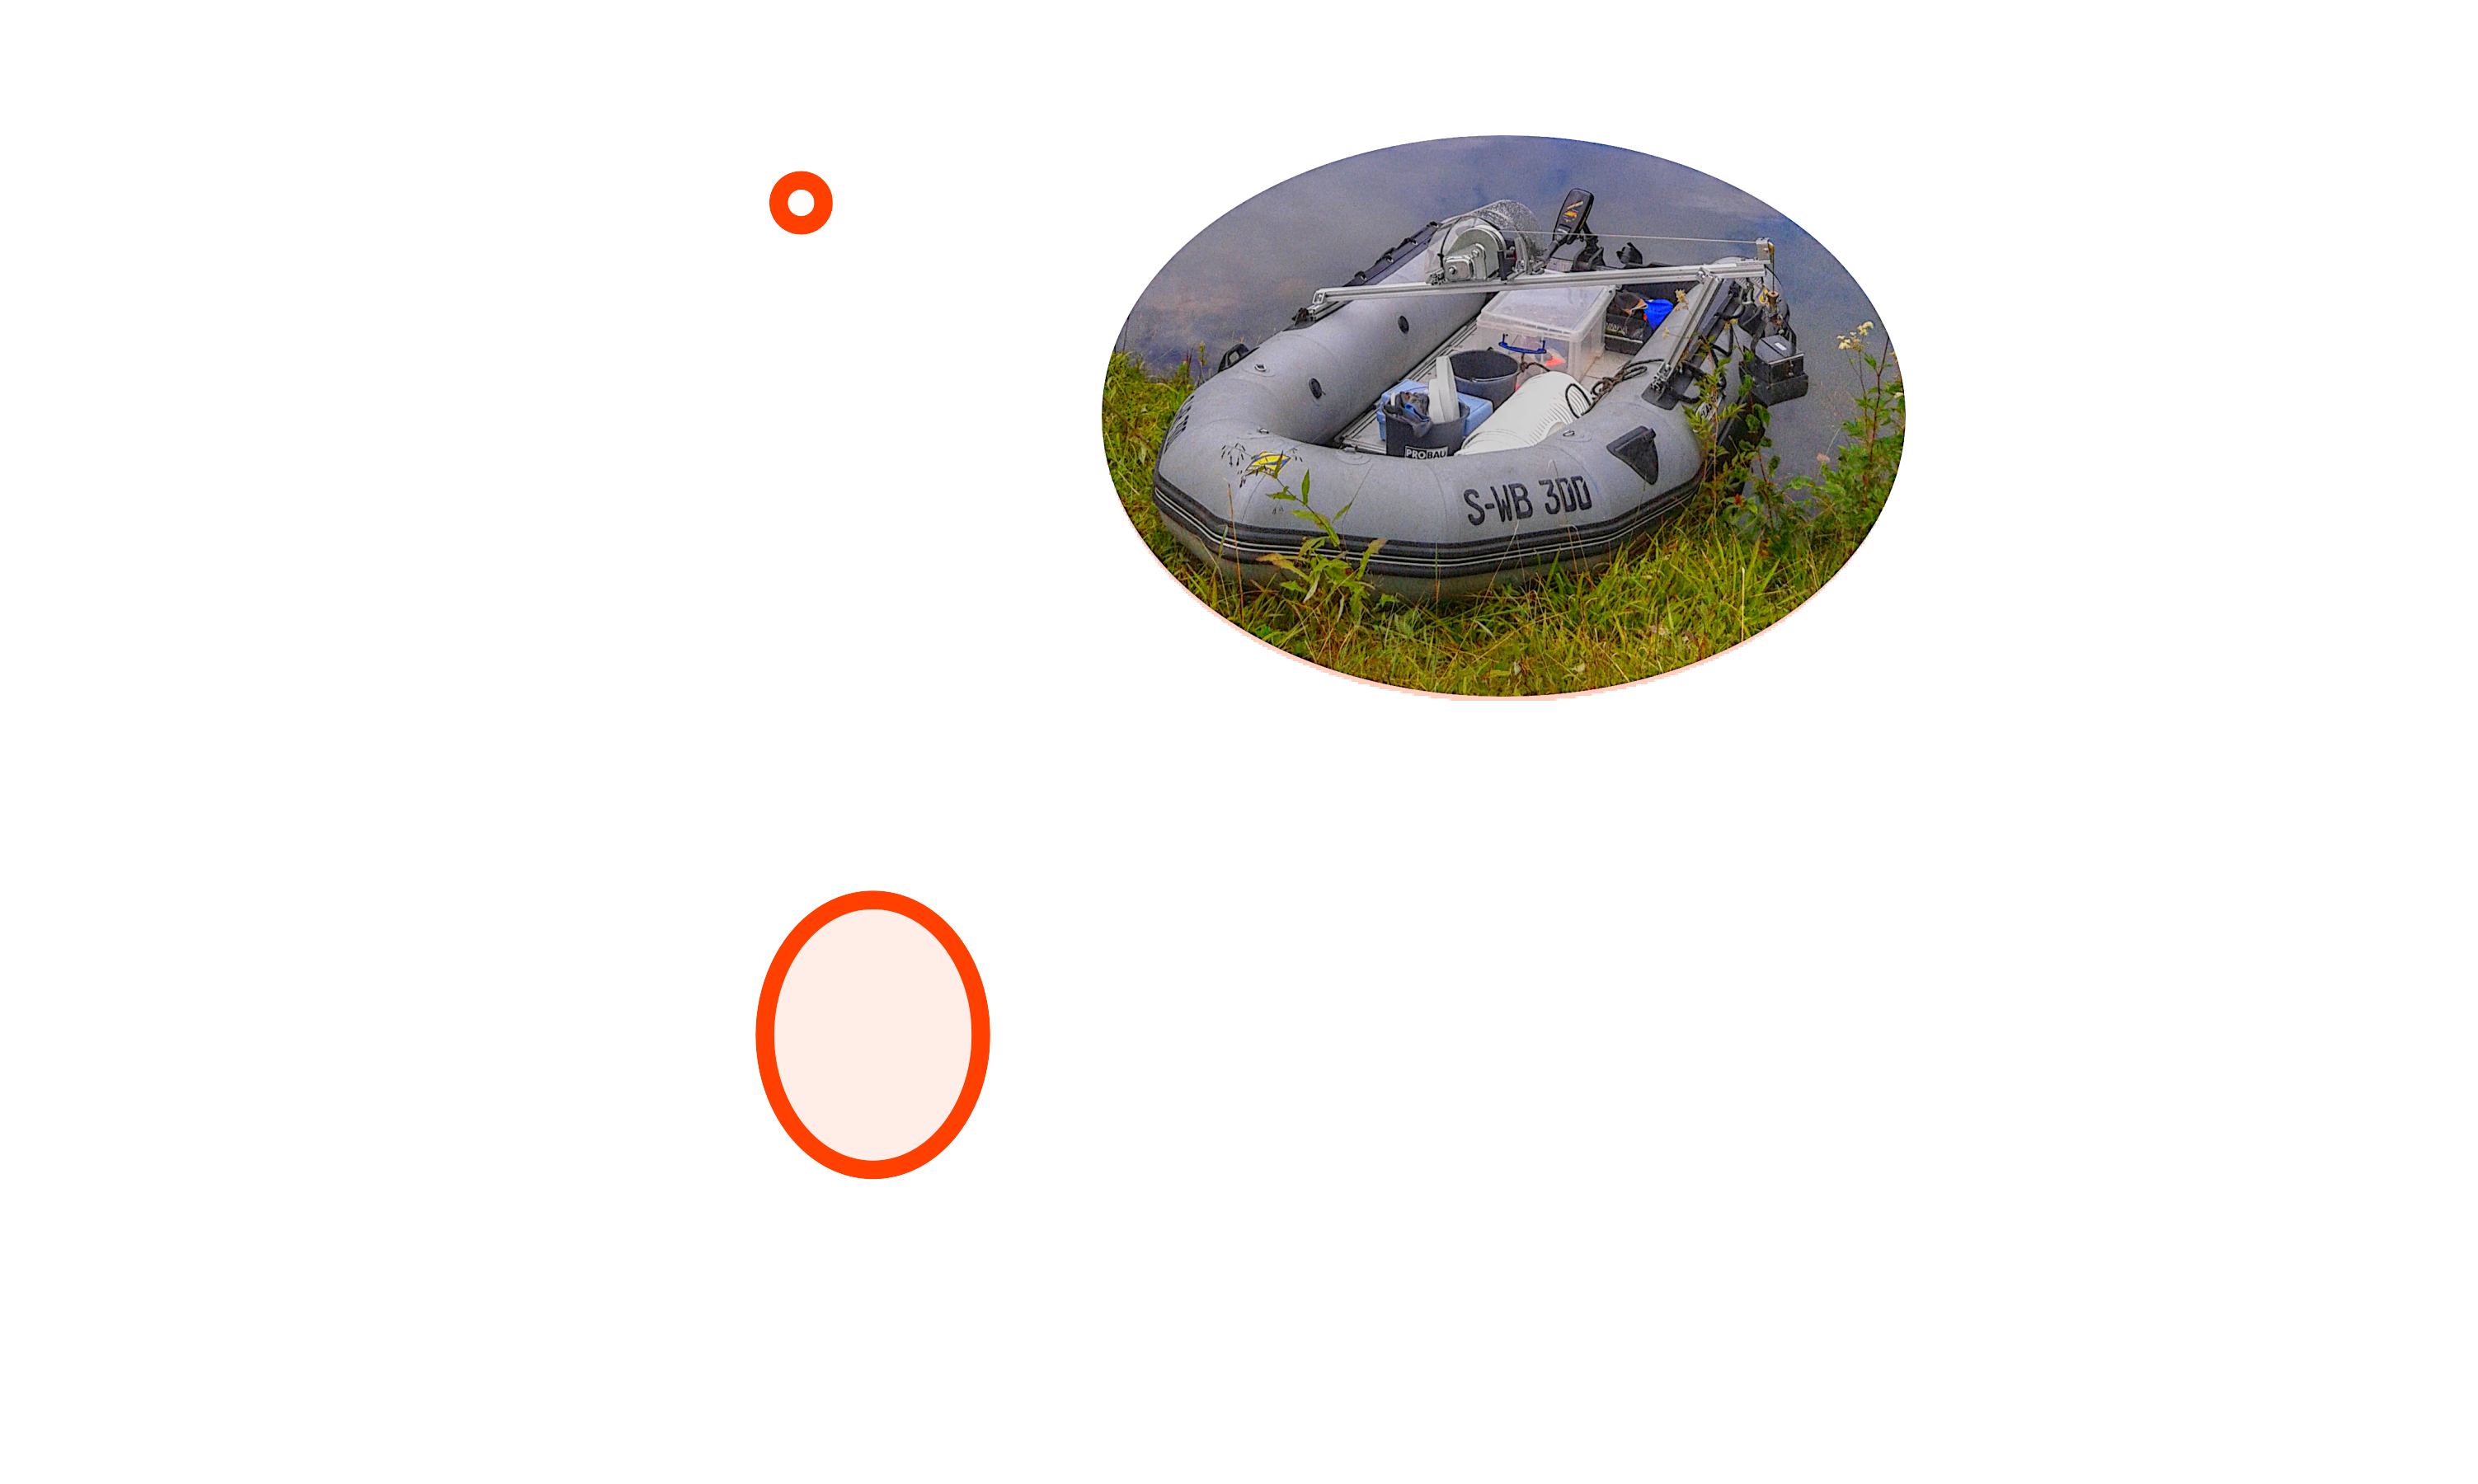
\includegraphics[width=0.88\paperwidth]{sbt-img-overlay}};
		\end{scope}}
		\onslide<1->{
			\node[anchor=south west, xshift=0.33\paperwidth, yshift=2.1947cm, text=black, text width=0.5\paperwidth,align=left]{\tiny \textcolor{gray}{Photography: IWS / Universität Stuttgart (2016)}};}
	\end{tikzpicture}
\end{frame}

\begin{frame}{\secname\vspace{0.1cm}\\\textcolor{anthrazit!80!white}{\subsecname}}
	Calibration of a Delft3D-FLOW model with:
	\begin{align*}
		\mbox{Measurement data}:= &\left[\begin{array}{ll}
		\textcolor{gray}{\mbox{water temperature in the reservoir}}~\mathbf{T}\\ \textcolor{gray}{\mbox{depth-averaged flow velocity}}~\mathbf{U} \end{array} \right]\hfill\\
		\mbox{Calibration parameters}  := &\left[\begin{array}{l}
			\textcolor{gray}{\mbox{background horizontal eddy viscosity}}~\nu^{back}_{h}\\
			\textcolor{gray}{\mbox{background horizontal eddy diffusivity}}~\Delta^{back}_{h}\\
			\textcolor{gray}{\mbox{water temperature at the inlet tower}}~T_{tow}
		\end{array}\right]\hfill
	\end{align*}
	\begin{tikzpicture}
		\clip (0,0) rectangle (\paperwidth,\paperheight);
		\onslide<2->{
		\begin{scope}
			\node[anchor=south west, xshift=0.0\paperwidth, yshift=0.543\paperheight] {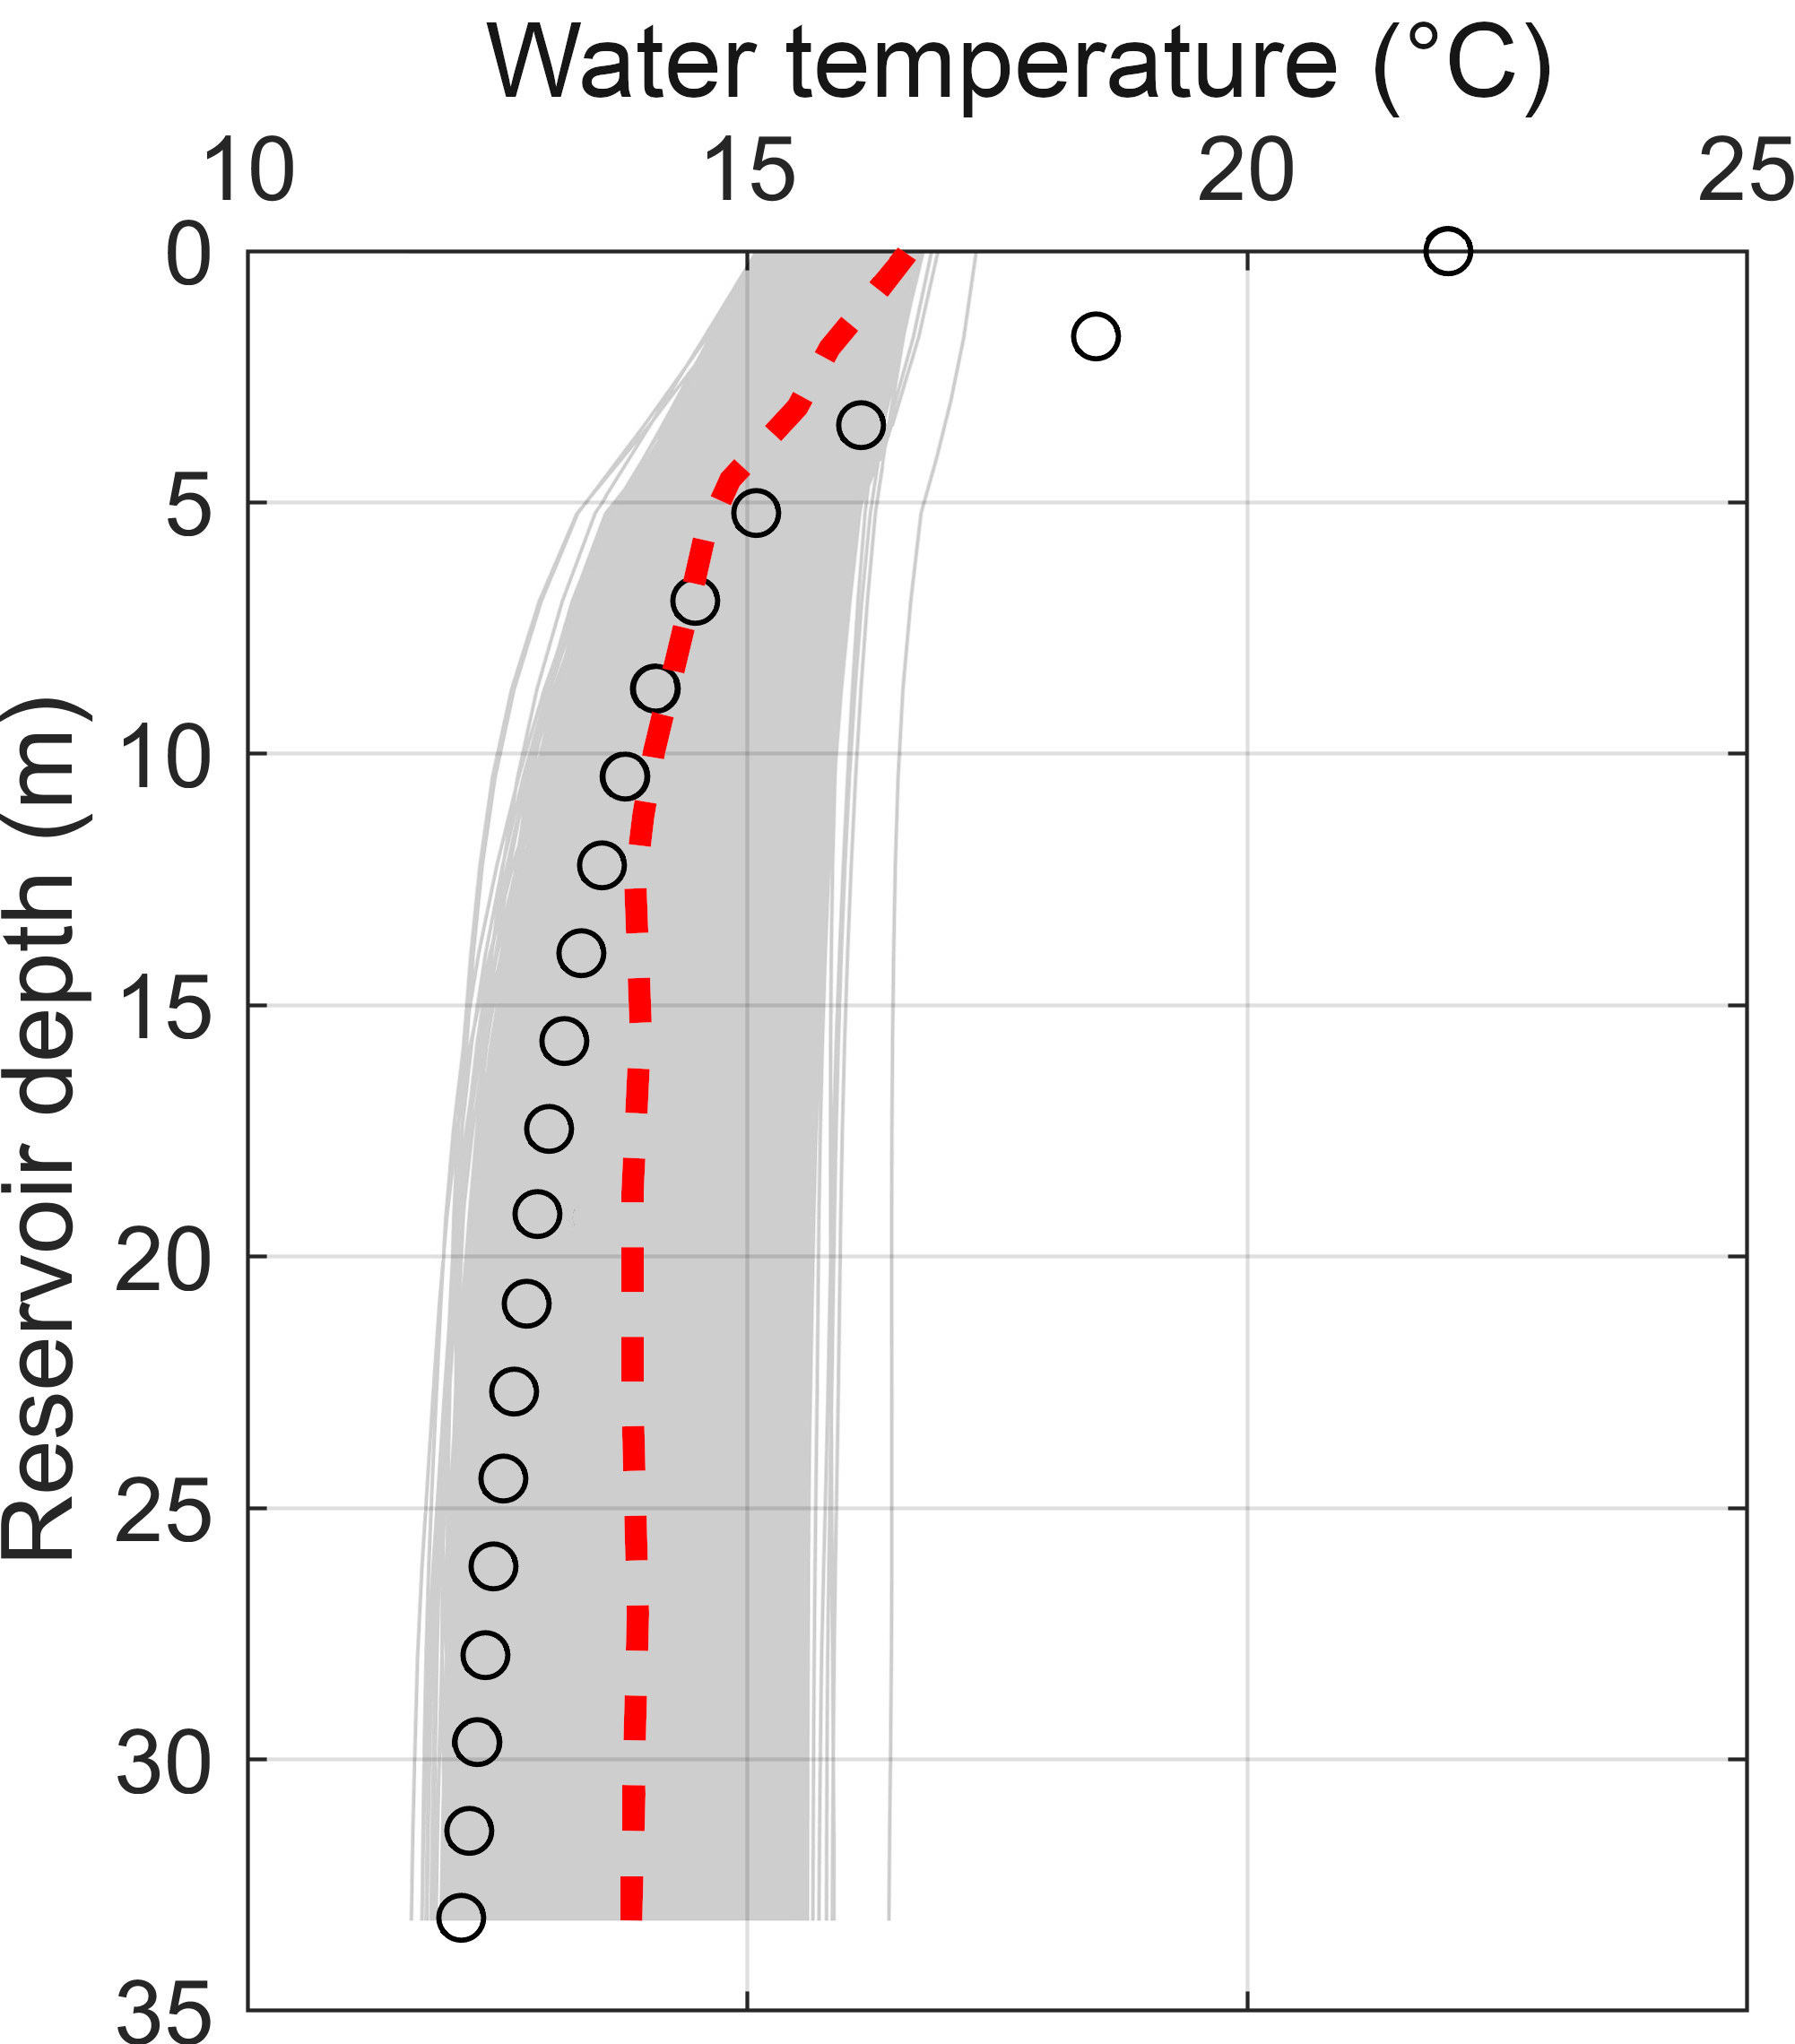
\includegraphics[height=0.434\paperheight]{sbt-water-temps-with-calib}};
		\end{scope}
		\begin{scope}
				\node[anchor=south west, xshift=0.3\paperwidth, yshift=0.5\paperheight] {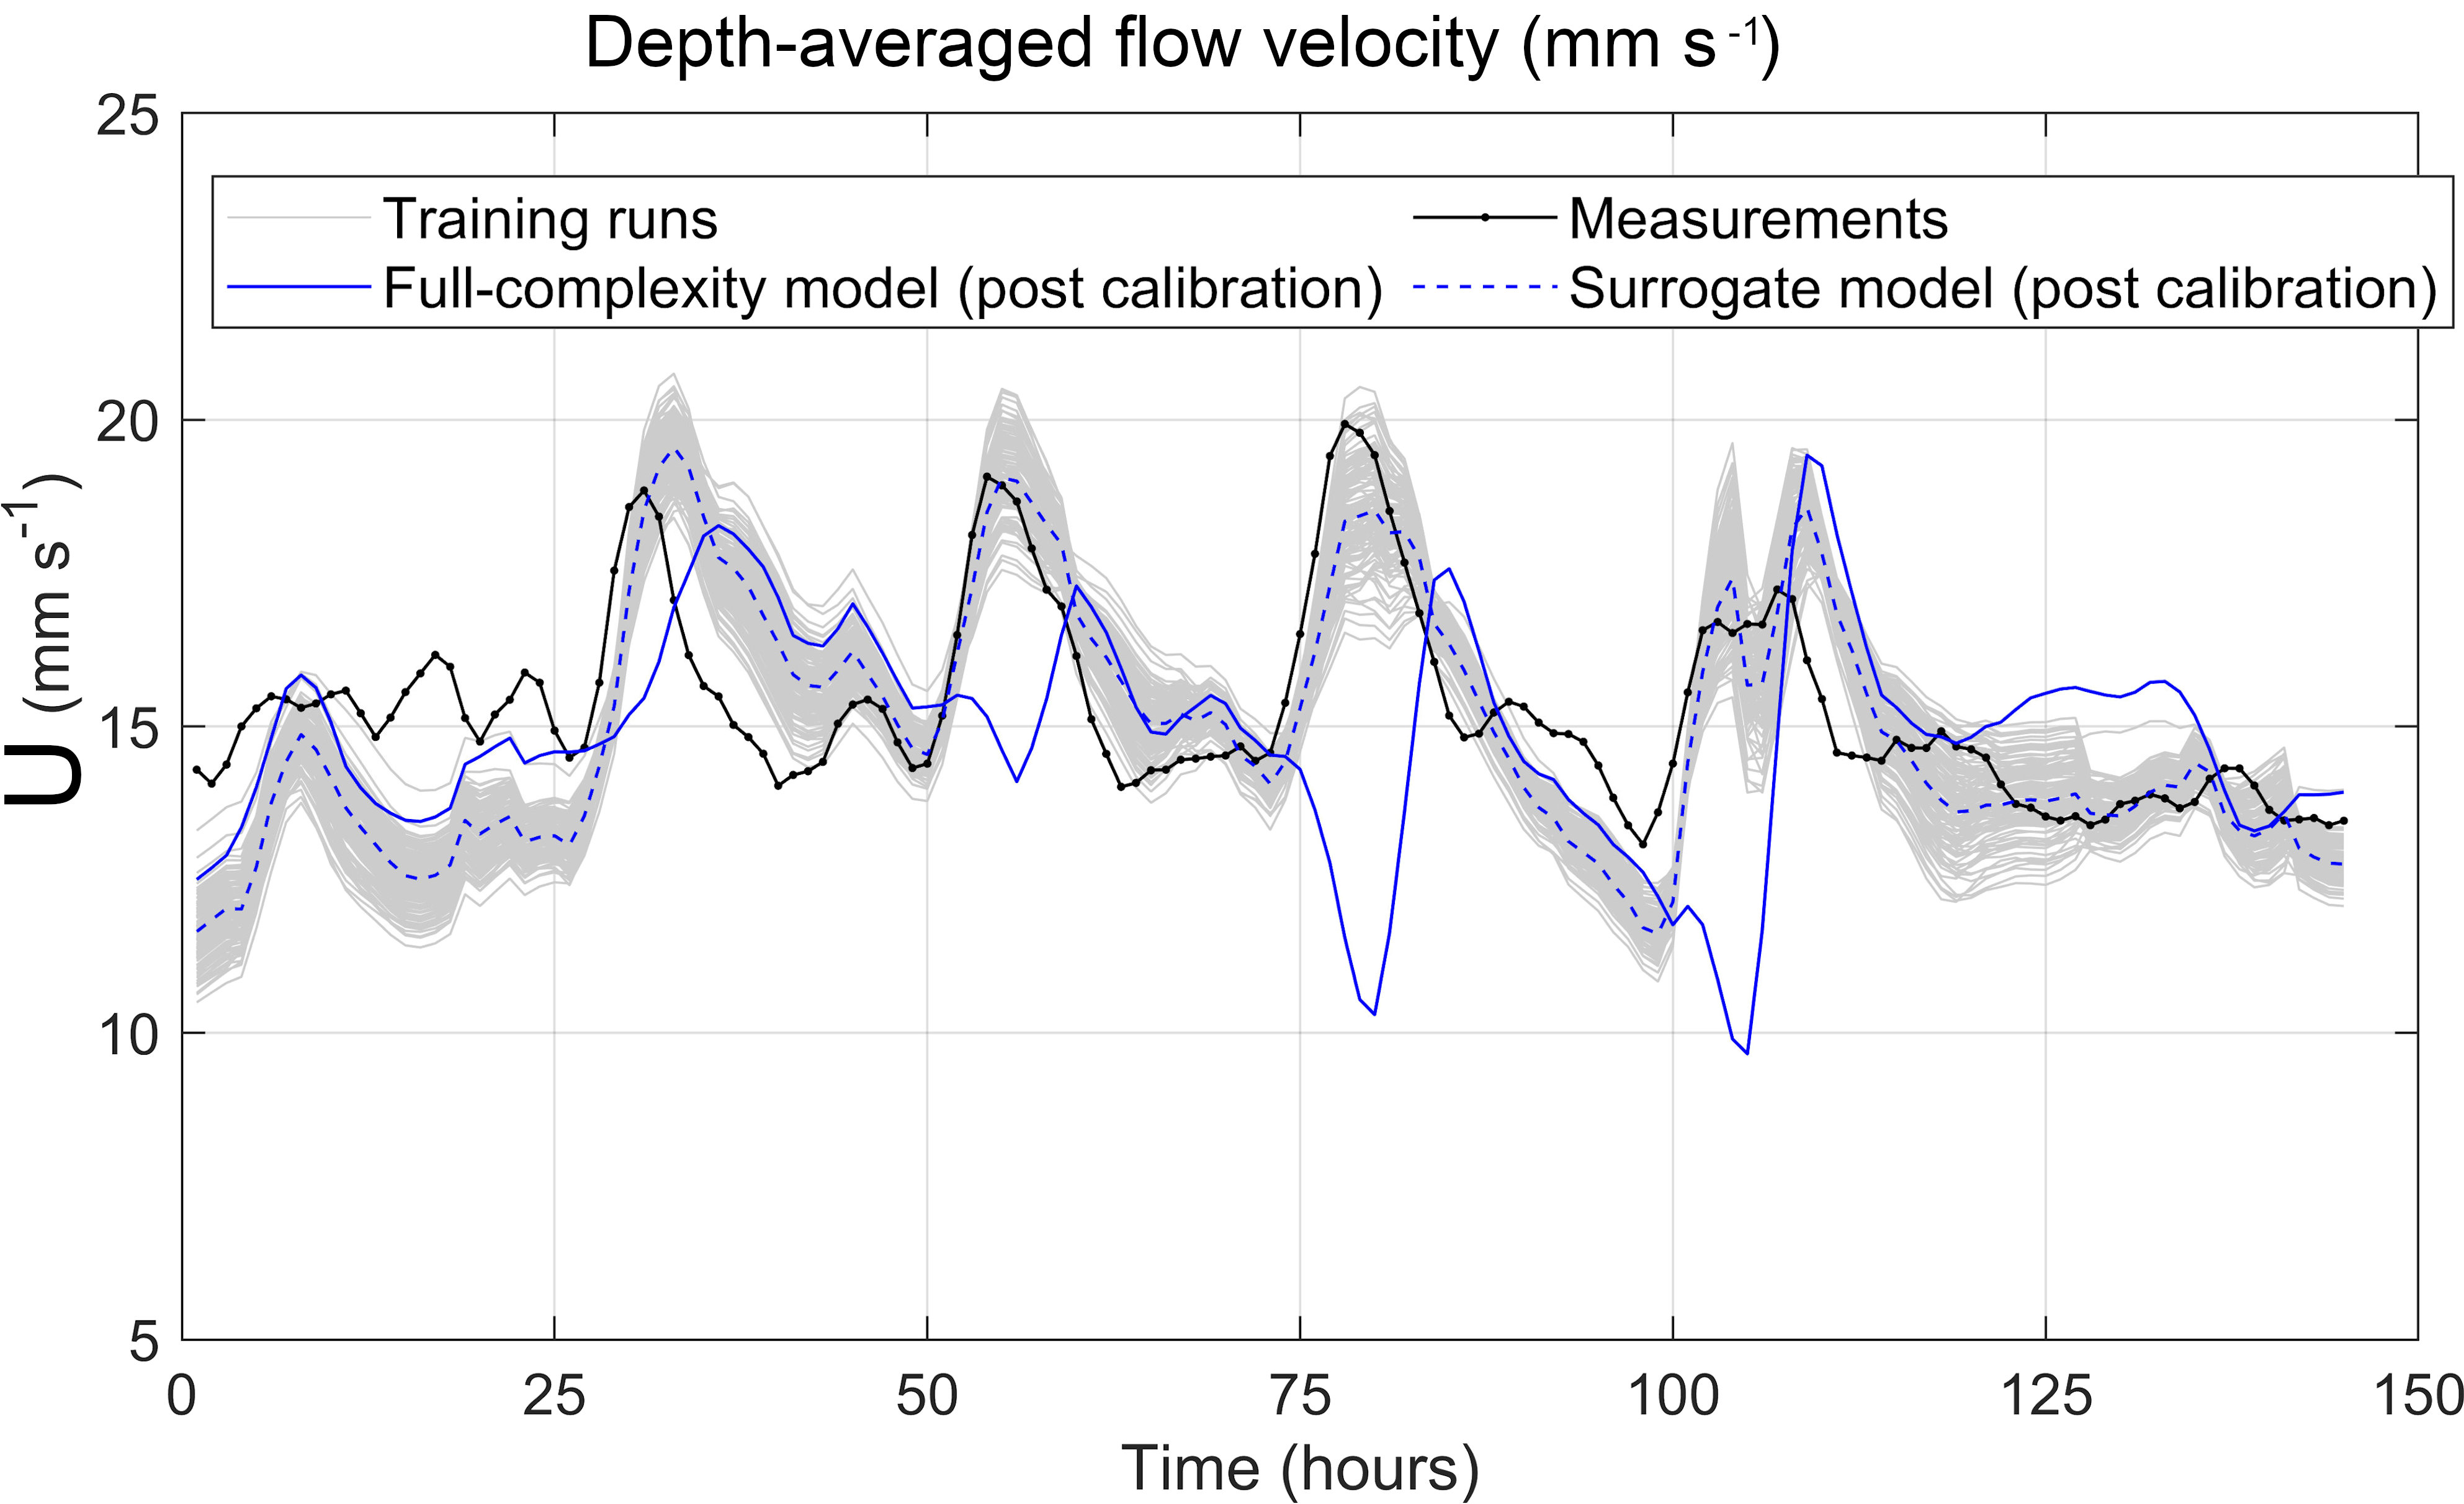
\includegraphics[height=0.4571578947368421\paperheight]{sbt-post-U-scenario0}};
		\end{scope}
		}
		\onslide<1->{
			\node[anchor=south west, xshift=0.33\paperwidth, yshift=4.43cm, text=black, text width=0.45\paperwidth,align=left]{\tiny \textcolor{gray}{Source: \sscURL{Schwindt \textit{et al.} (2023)}{https://doi.org/10.1029/2022WR033660}}};}
		\onslide<3->{
			\fill[unisblue,opacity=0.95,xshift=-0.57\paperwidth,yshift=0.63] (\paperwidth,0.63\paperheight) circle (0.35\paperheight);
			% place text in circle
			\node at (\paperwidth,0.665\paperheight)[xshift=-0.57\paperwidth,yshift=0.665,text width=0.45\paperwidth,align=center]{\huge {\textcolor{white}{RMSE ($\mathbf{T}$)~=~1.76$^{\circ}$C\\RMSE ($\mathbf{U}$)~=~1.43 mm s$^{-1}$\vspace{0.2cm}\\
						\onslide<4->{\textbf{Great model?}\\\textbf{NO!}}}\par}};
		}
	\end{tikzpicture}
\end{frame}

\begin{frame}{\secname\vspace{0.1cm}\\\textcolor{anthrazit!80!white}{\subsecname}}
	\begin{tikzpicture}
		\clip (0,0) rectangle (\paperwidth,\paperheight);
		\onslide<1->{
		\begin{scope}
			\node[anchor=south west, xshift=0.05\paperwidth, yshift=0.52\paperheight] {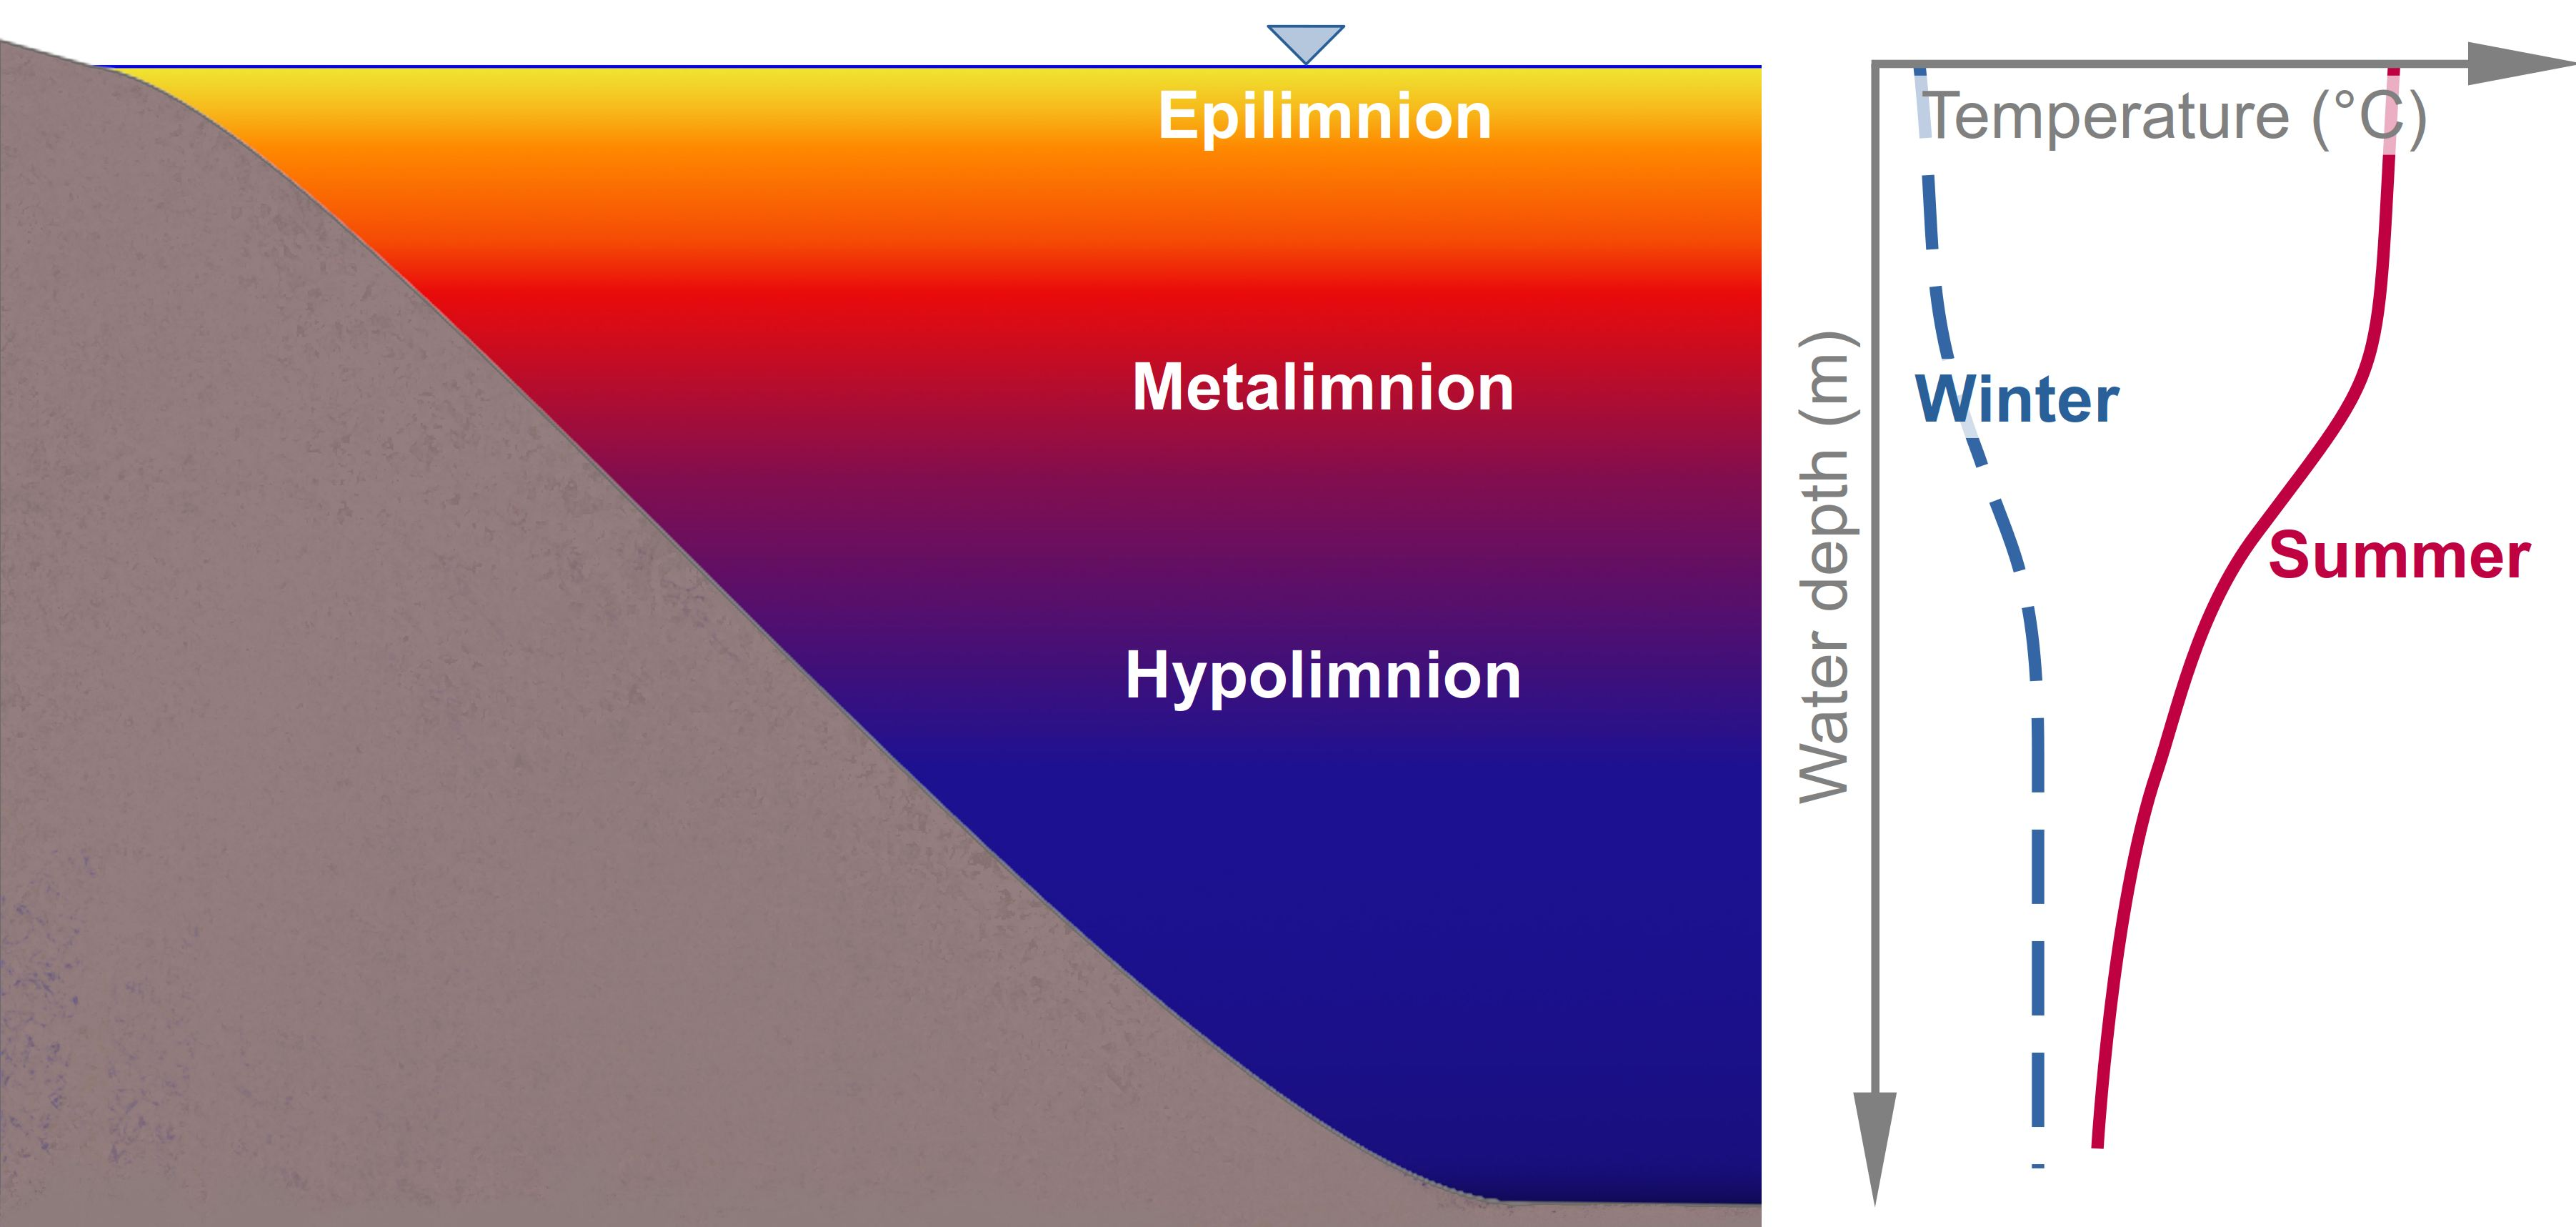
\includegraphics[width=0.75	\paperwidth]{stratification}};
		\end{scope}}
		\begin{scope}
			\node[anchor=south west, xshift=0.0\paperwidth, yshift=0.3\paperheight] {
				\begin{minipage}{0.95\textwidth}
					\begin{itemize}
						\item[\faHandORight] Seasonal stratification of the Schwarzenbach reservoir sets in after \textbf{several weeks}
						\onslide<2->{
							\item[\faHandORight] The numerical model \textbf{forced stratification in 6 days}
							\item[\faHandORight] Water temperature measurements \textbf{confused supervised learning}
						}
					\end{itemize}
				\end{minipage}
			};
		\end{scope}
	\end{tikzpicture}
\end{frame}

\begin{frame}{\secname\vspace{0.1cm}\\\textcolor{anthrazit!80!white}{\subsecname}}\vspace{-0.2cm}
	\begin{center}
		\textcolor{unisblue}{\textbf{Characteristics of confused Bayesian calibration\onslide<2->{: high uncertainty}}}
	\end{center}	
	\begin{tikzpicture}
		\clip (0,0) rectangle (\paperwidth,\paperheight);
		\onslide<1->{
			\begin{scope}
				\node[anchor=south west, xshift=0.05\paperwidth, yshift=0.32\paperheight] {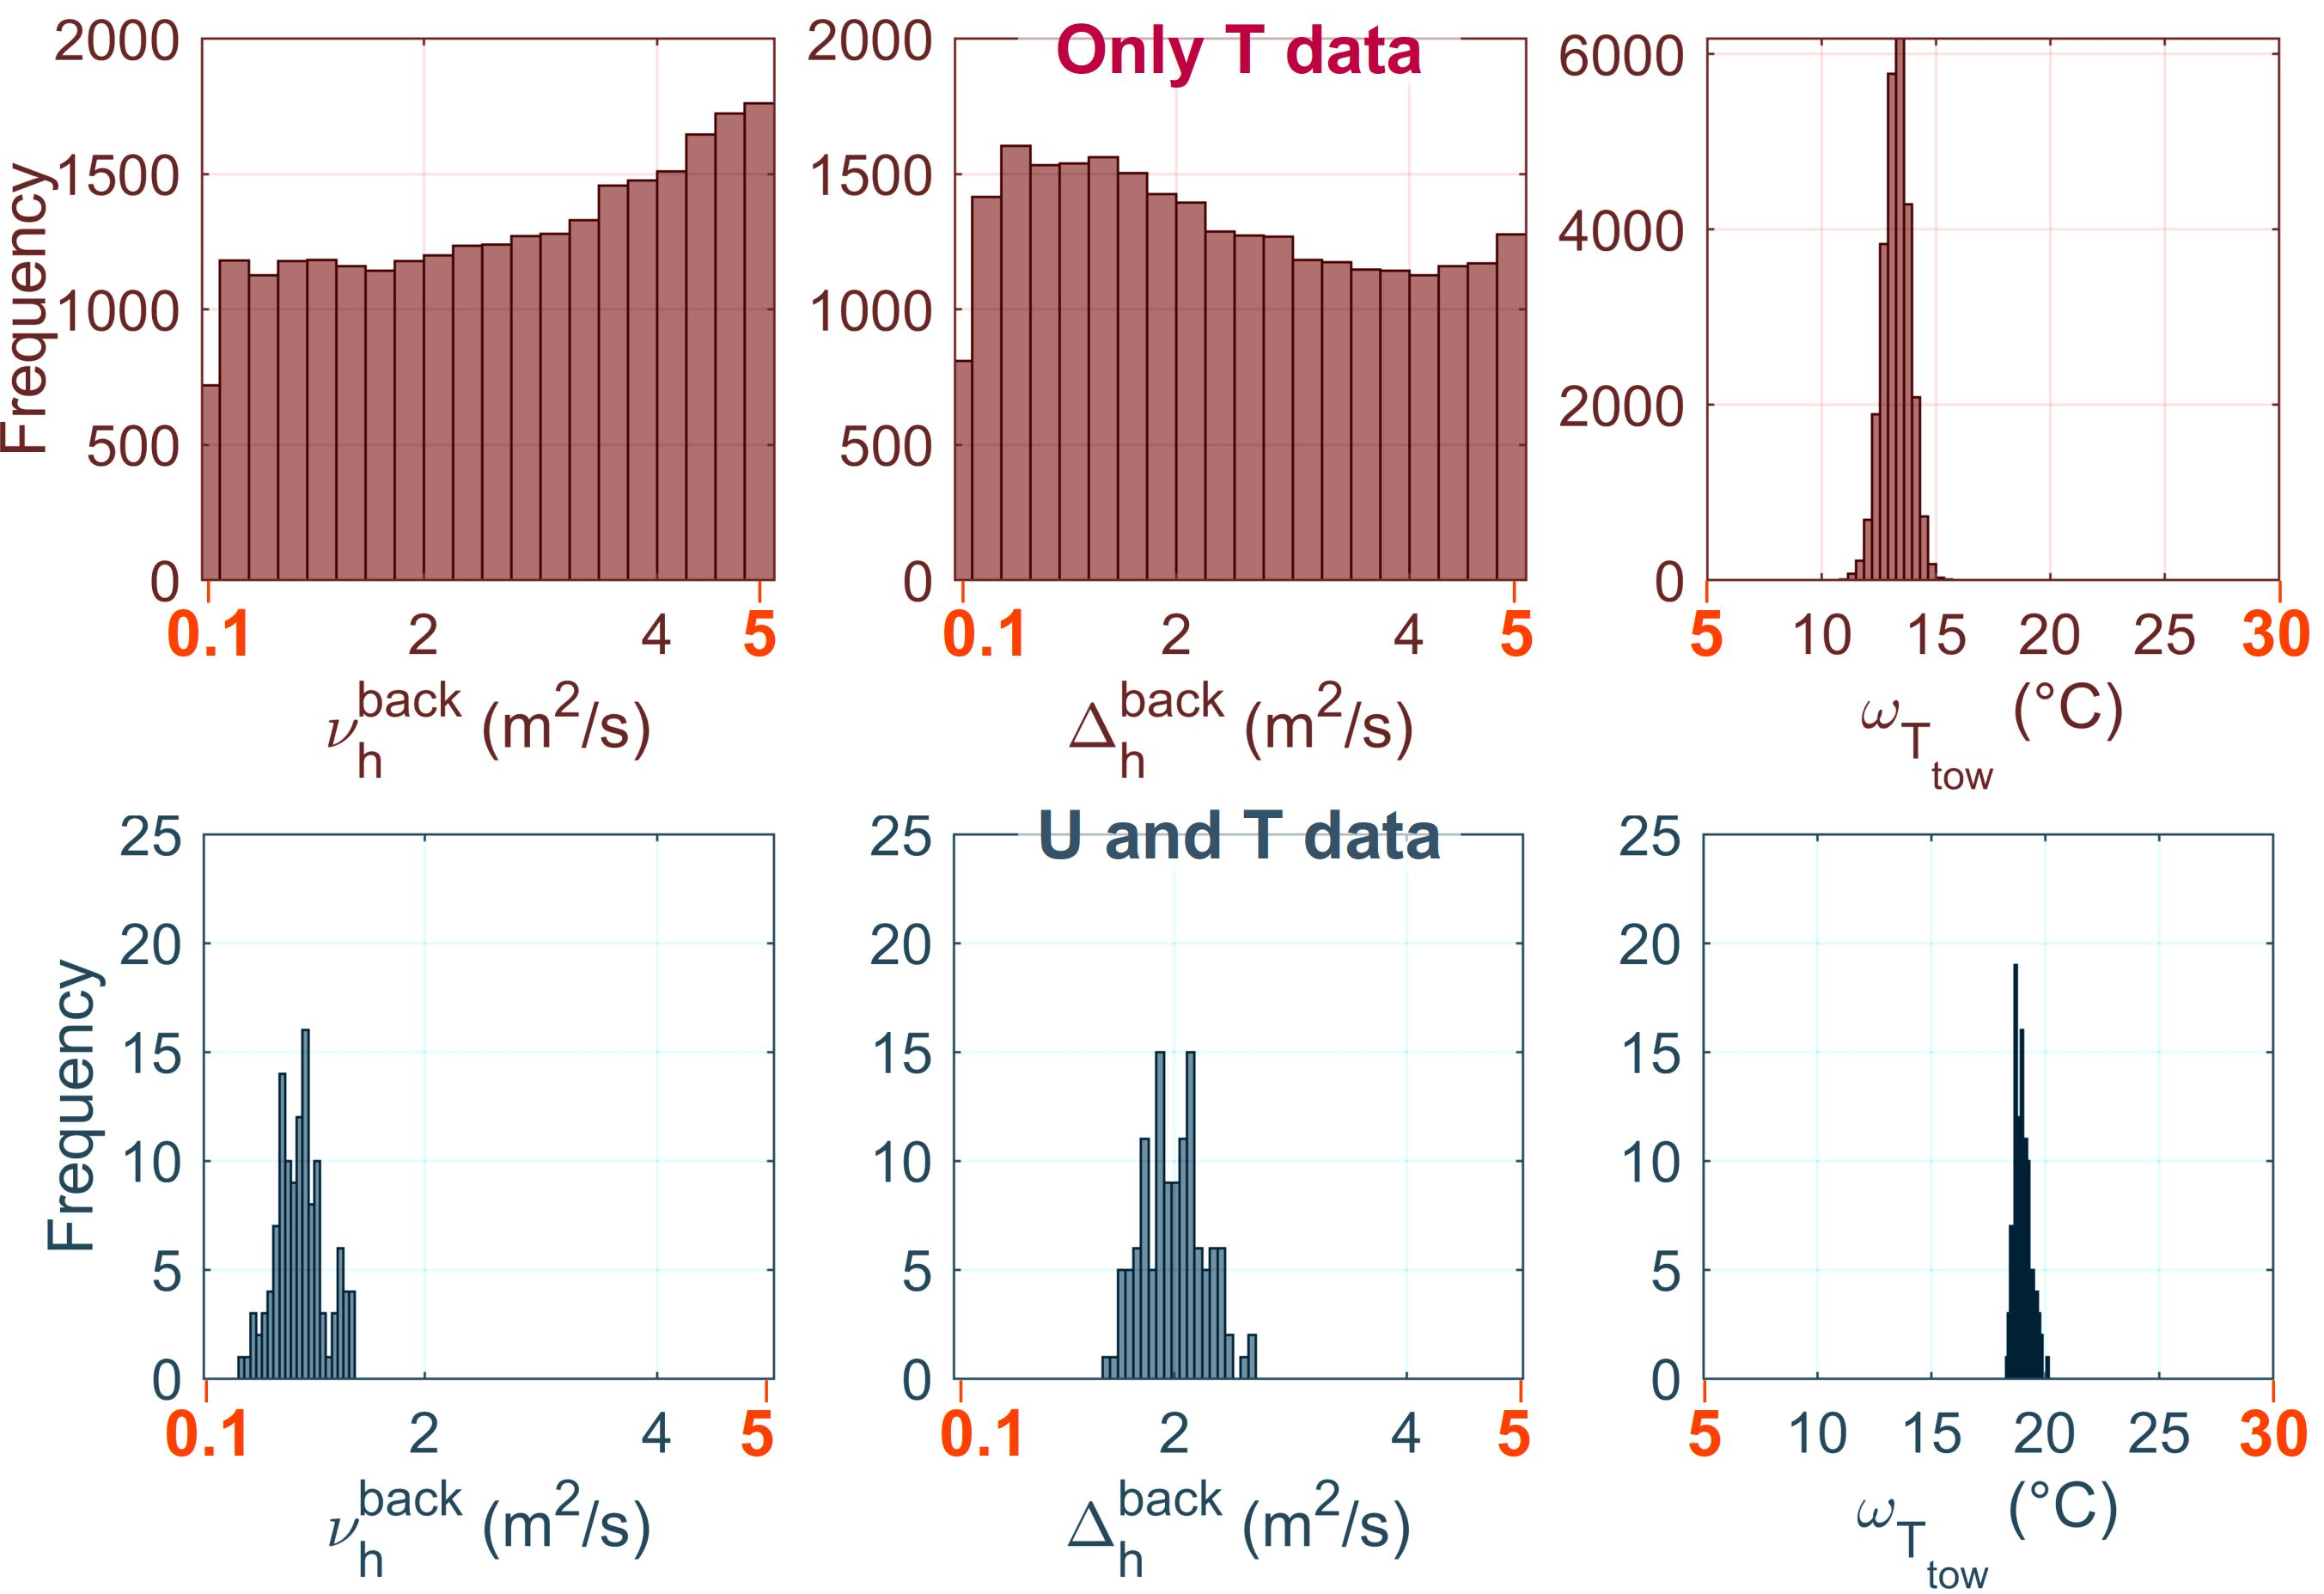
\includegraphics[width=0.73	\paperwidth]{sbt-uncertainty}};
		\end{scope}}
		\onslide<2->{
		\begin{scope}
			\node[anchor=south west, xshift=0.05\paperwidth, yshift=0.32\paperheight] {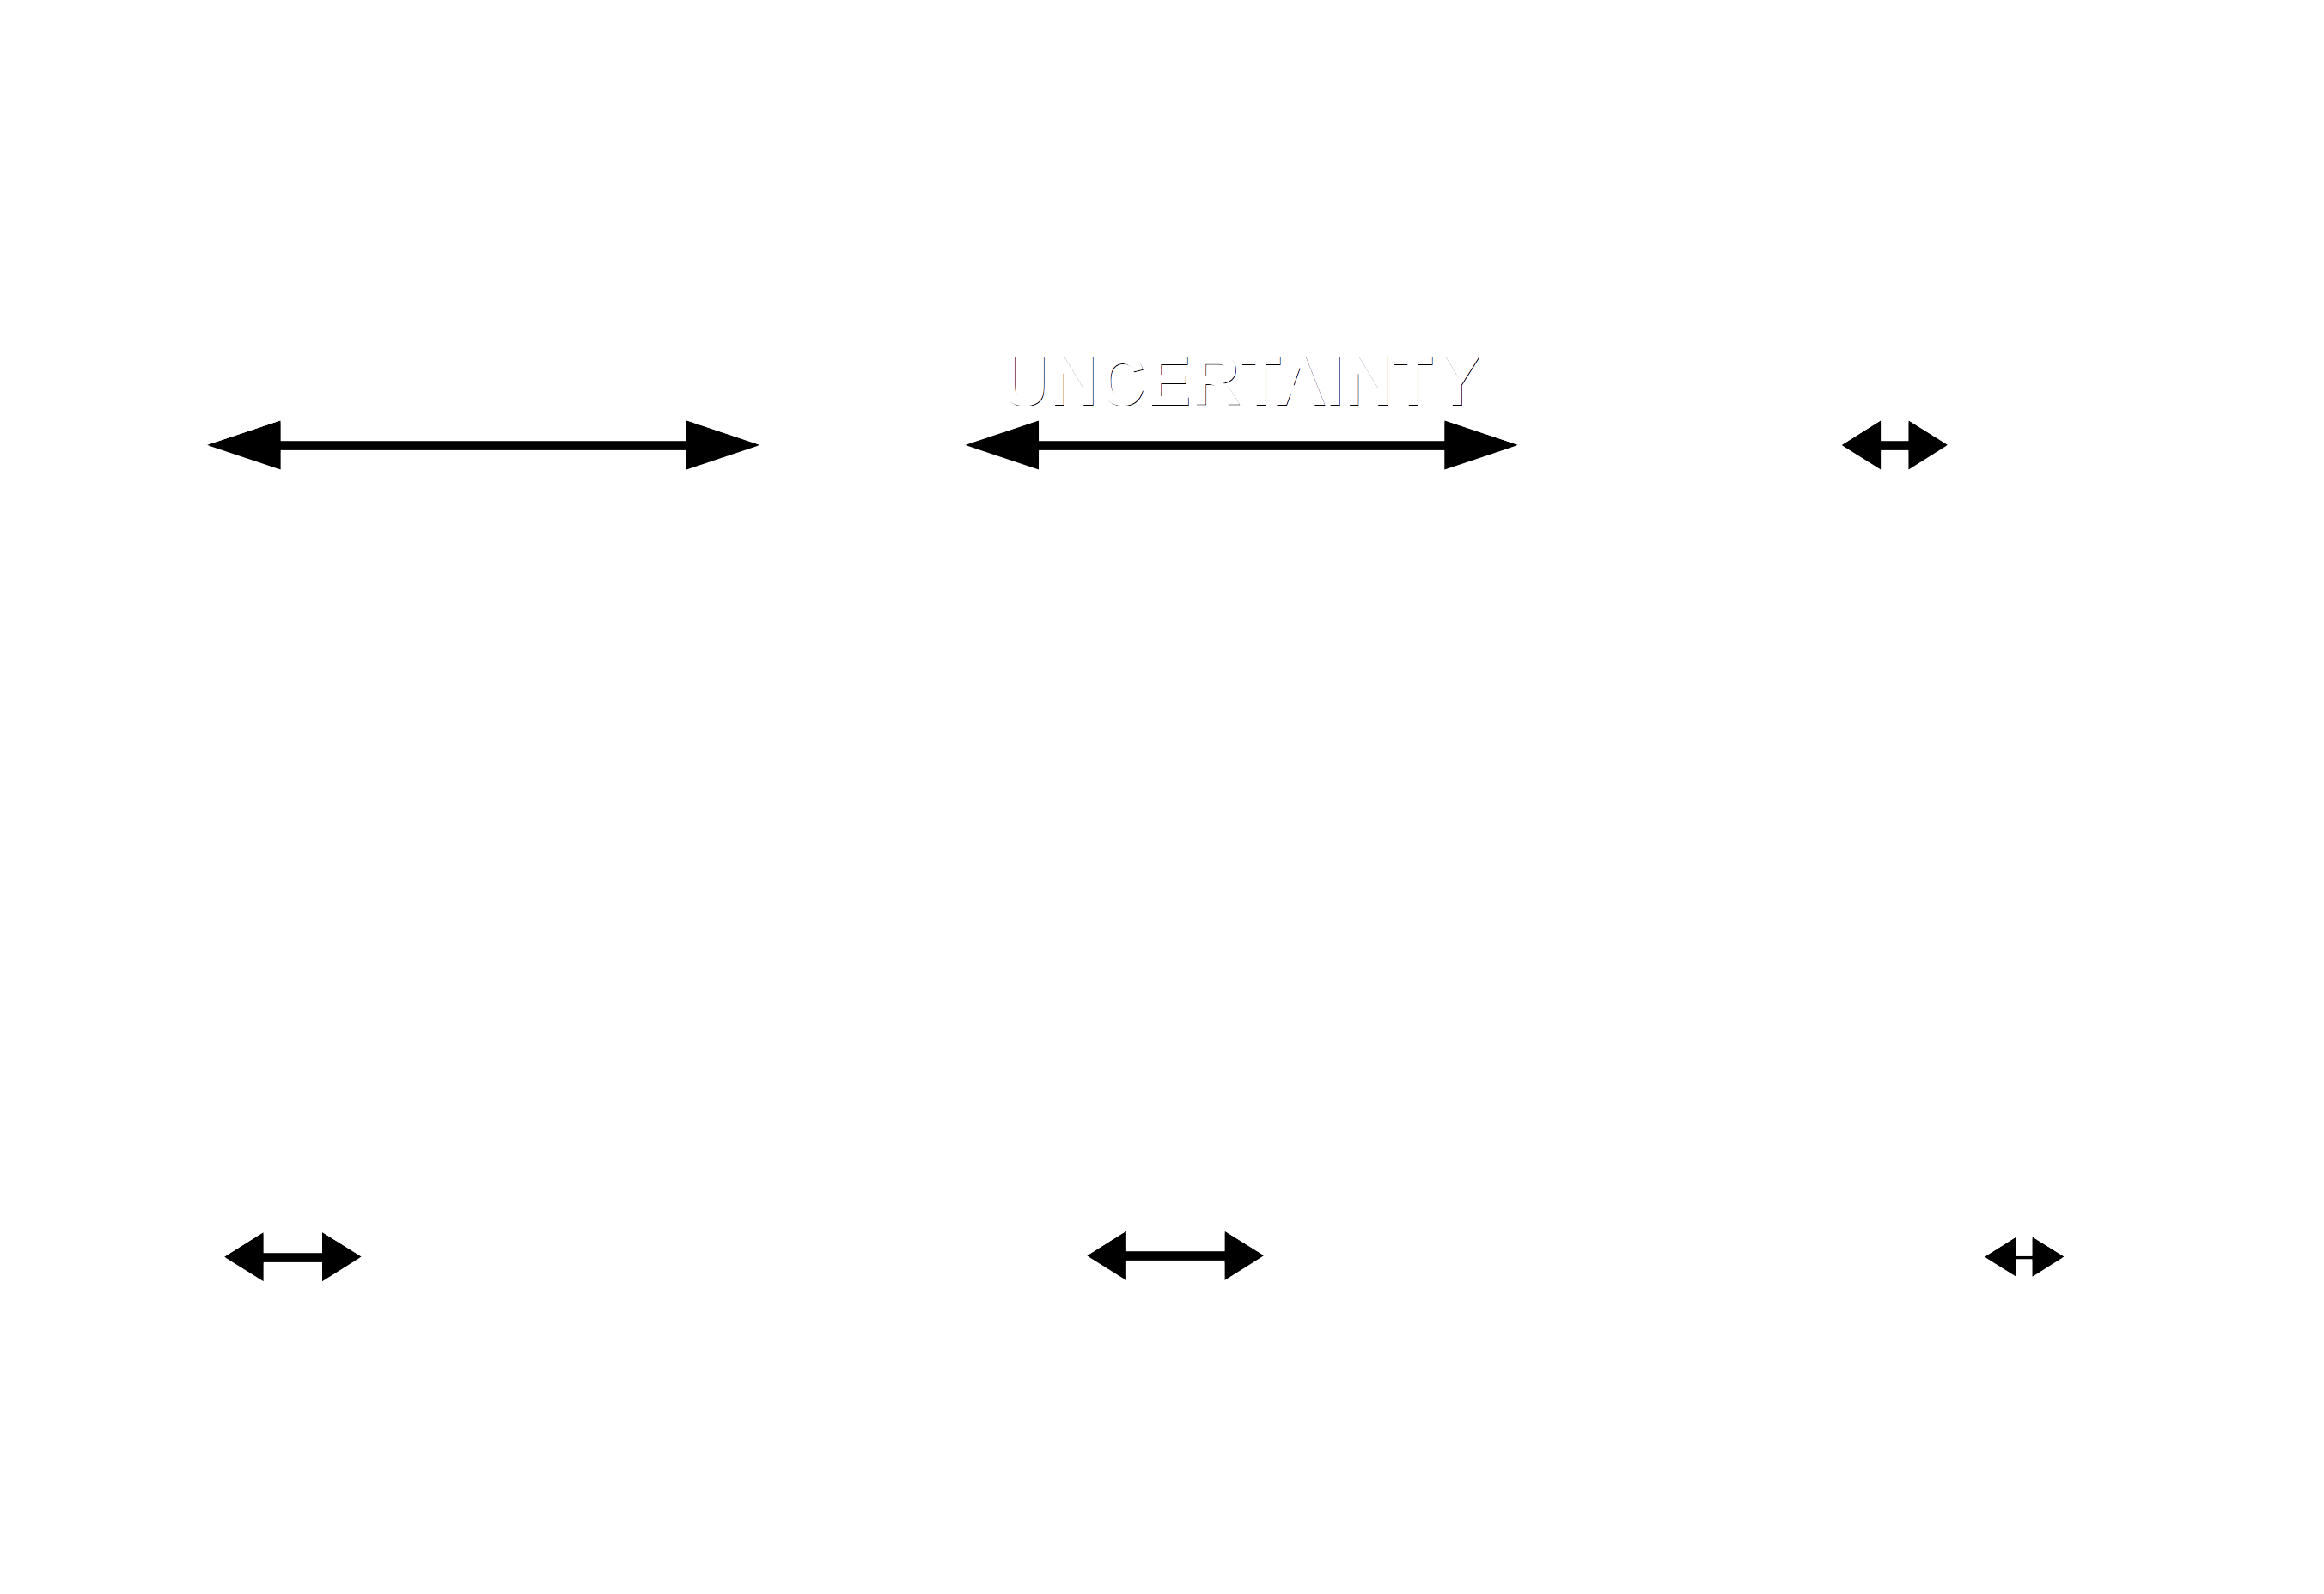
\includegraphics[width=0.73	\paperwidth]{sbt-uncertainty-overlay}};
		\end{scope}}
		\onslide<1->{
			\node[anchor=south west, xshift=0.33\paperwidth, yshift=2.606cm, text=black, text width=0.45\paperwidth,align=left]{\tiny \textcolor{gray}{Source: \sscURL{Schwindt \textit{et al.} (2023)}{https://doi.org/10.1029/2022WR033660}}};}
	\end{tikzpicture}
\end{frame}

\subsection{Steps Toward Solutions}
\begin{frame}{\secname\vspace{0.1cm}\\\textcolor{anthrazit!80!white}{\subsecname}}%\vspace{.1cm}
	\begin{tikzpicture}
	\clip (0,0) rectangle (\paperwidth,\paperheight);
	\onslide<1->{
		\begin{scope}
			\node[anchor=south west, xshift=0.05\paperwidth, yshift=0.4\paperheight] {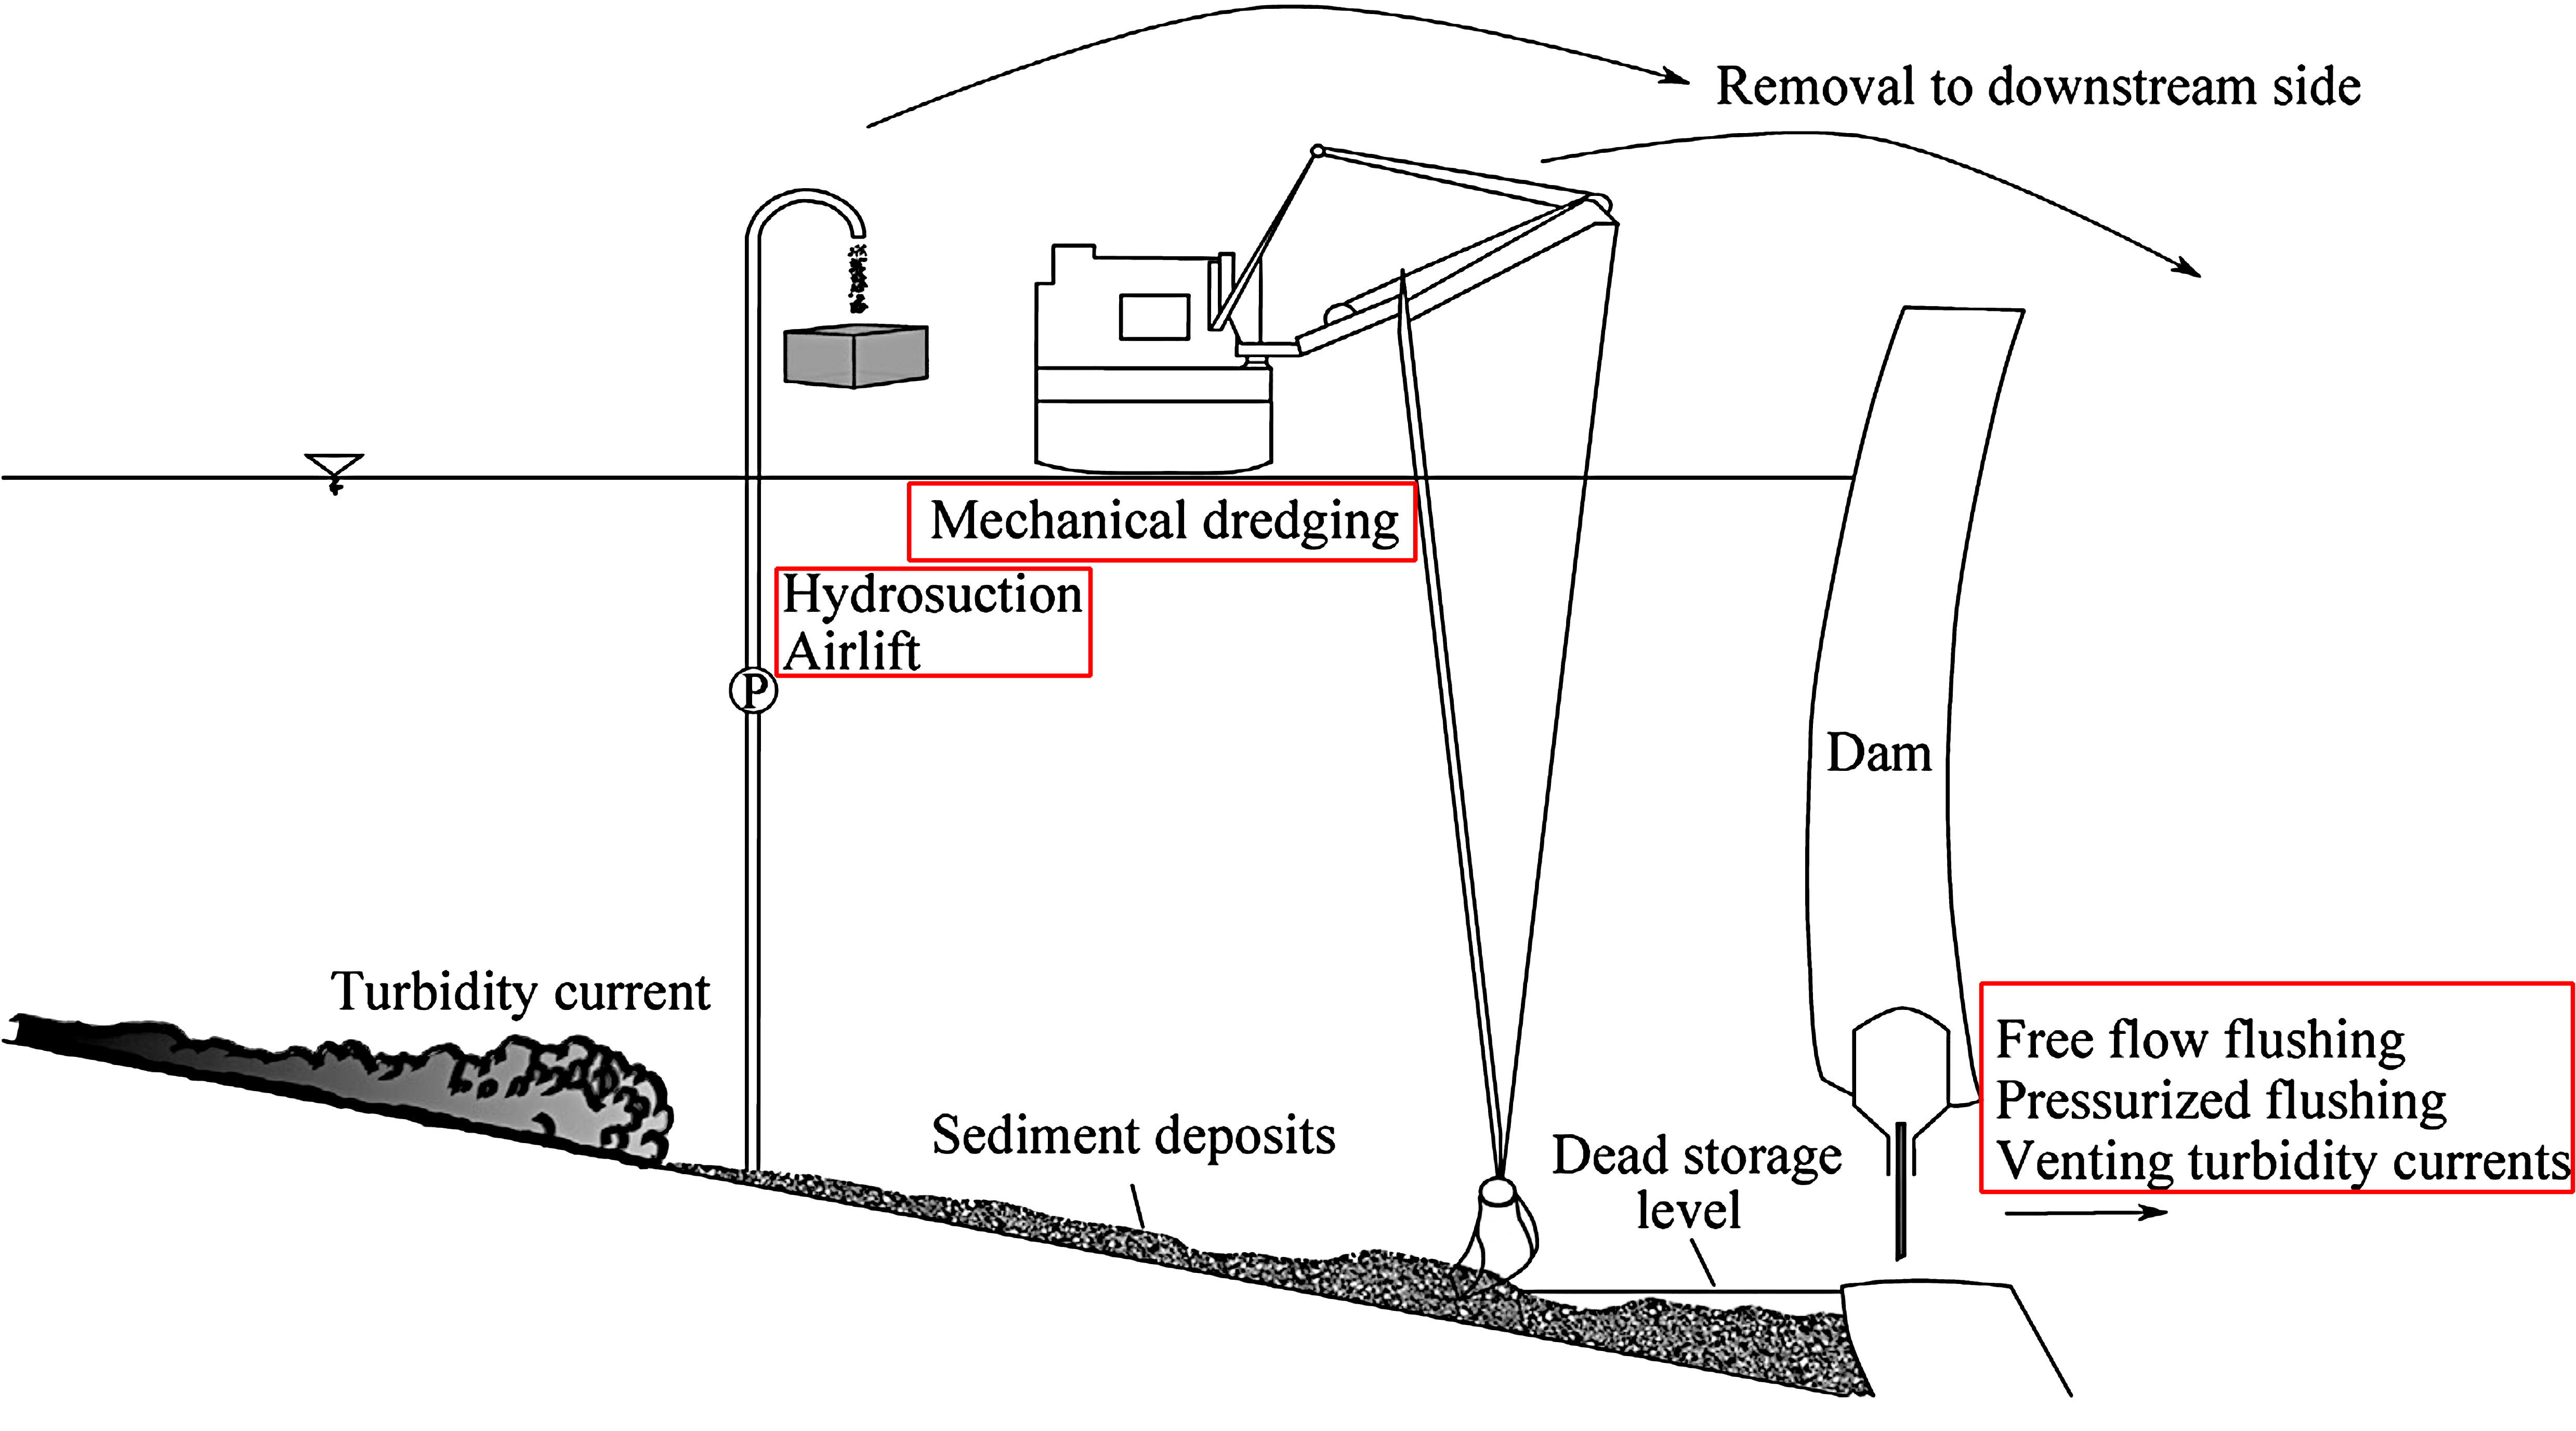
\includegraphics[width=0.78	\paperwidth]{reservoir-sedimentation-mgmt-highlight}};
	\end{scope}}
	\onslide<1->{
		\begin{scope}
			\node[anchor=south west, xshift=0.0\paperwidth, yshift=0.3\paperheight] {
				\begin{minipage}{0.95\textwidth}
					\begin{itemize}
						\item[\faHandORight]\ Airlift / hydrosuction
						\item[\faHandORight]\ Mechanical dredging
						\item[\faHandORight]\ Flushing (free flow, pressurized, venting) \& re-suspension
						\item[\faHandORight]\ Sediment bypass tunnels
					\end{itemize}
				\end{minipage}
			};
	\end{scope}}
	\onslide<1->{
		\begin{scope}
			\node[opacity=0.9, anchor=south west, xshift=0.0\paperwidth, yshift=0.1\paperheight] {
\includegraphics[width=\paperwidth]{white}};
		\end{scope}
		\node at (\paperwidth,0.86\paperheight)[xshift=-0.57\paperwidth,yshift=0.8,text width=0.89\paperwidth,align=center]{
		\begin{minipage}{0.95\textwidth}
		\begin{tcolorbox}[colbacktitle=hellblau!80!black, colback=hellblau!40!white, fonttitle=\bfseries, standard jigsaw,colframe=blue_light, bottom=0mm, middle=0mm, boxsep=0.2mm, opacityframe=0.5, opacityfill=0.7, opacitybacktitle=0.95, title filled, title={\faGraduationCap\ Bayesian calibration of numerical models}, size=fbox]
			\vspace{0.25cm}		 
			\begin{itemize}			
				\item[\faCheckSquareO] Innovative technique for improved accuracy enabled by thousands of surrogate model runs to identify \textbf{uncertainty}
				\item[\faCheckSquareO] \textbf{Higher} statistical \textbf{accuracy} provides better predictions for implementing \& optimizing sediment transfer solutions
			\end{itemize}
			\vspace{0.1cm}
		\end{tcolorbox}%\smallskip
		\end{minipage}
		};
	}
	\onslide<2->{
		\begin{scope}
			\node[anchor=south west, xshift=0.0\paperwidth, yshift=0.28\paperheight] {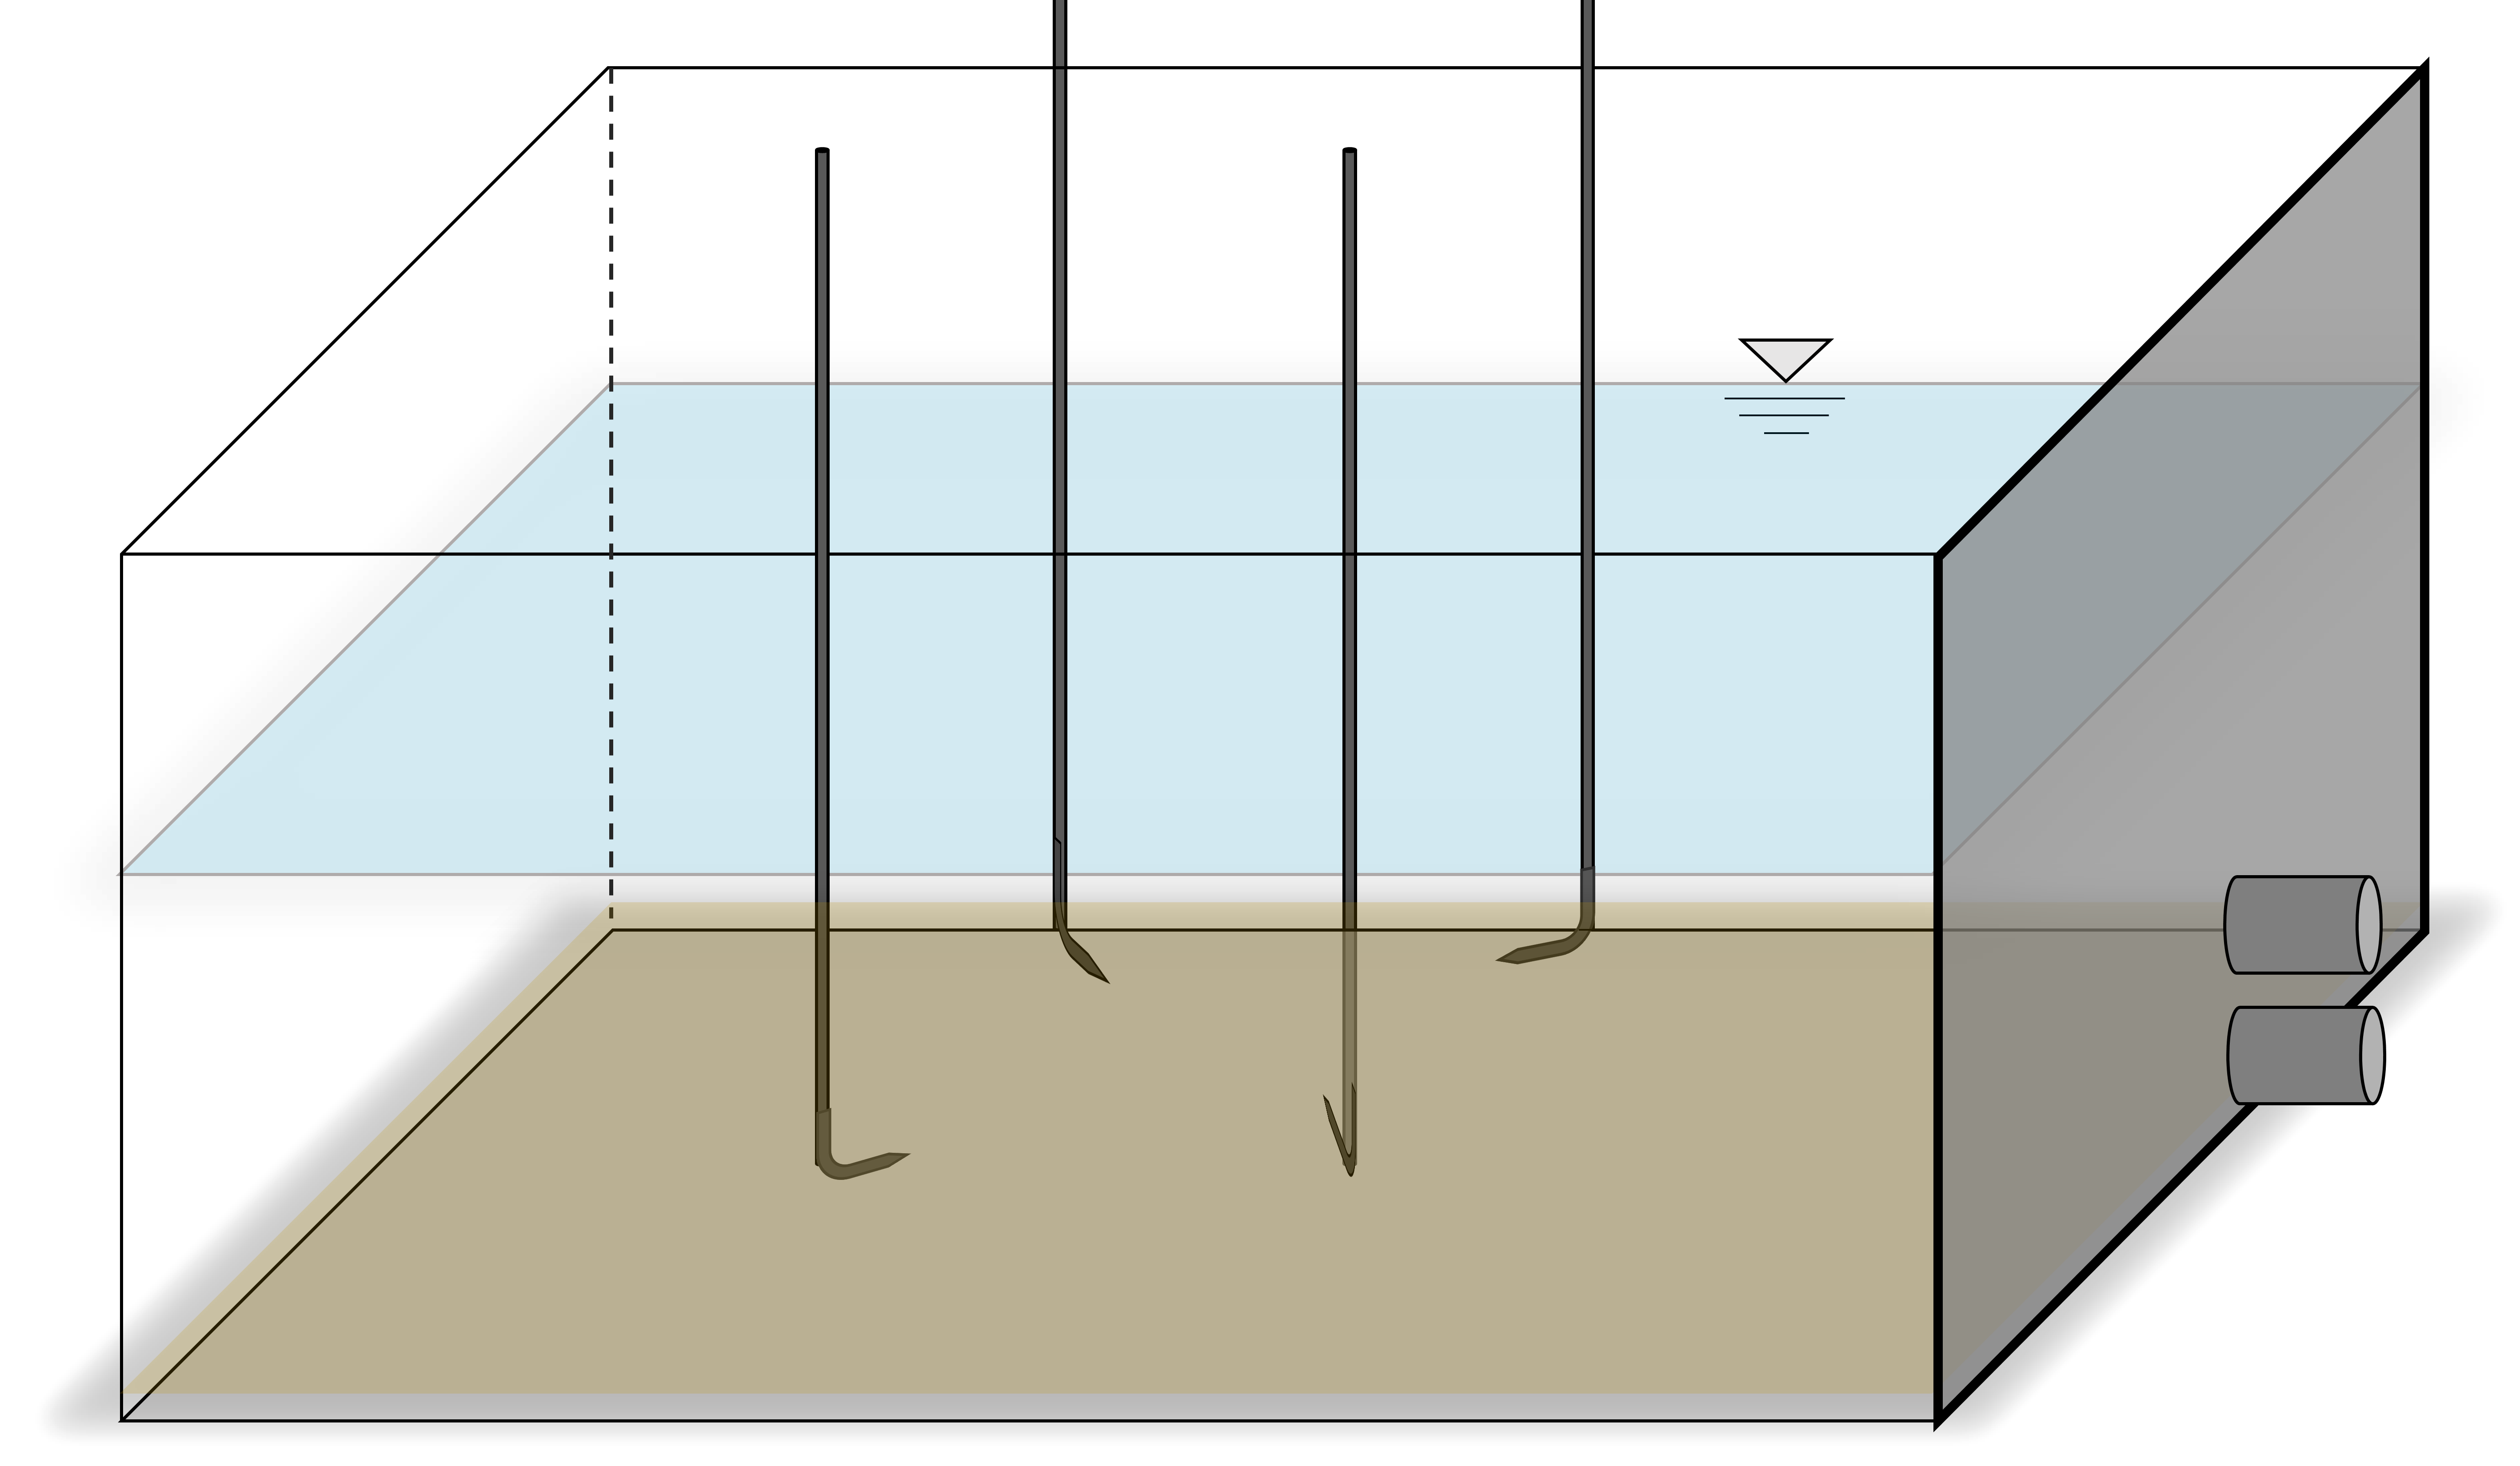
\includegraphics[height=0.4\paperheight]{jenzer-resuspend}};
		\end{scope}
		\begin{scope}
			\node[anchor=south west, xshift=0.54\paperwidth, yshift=0.285\paperheight] {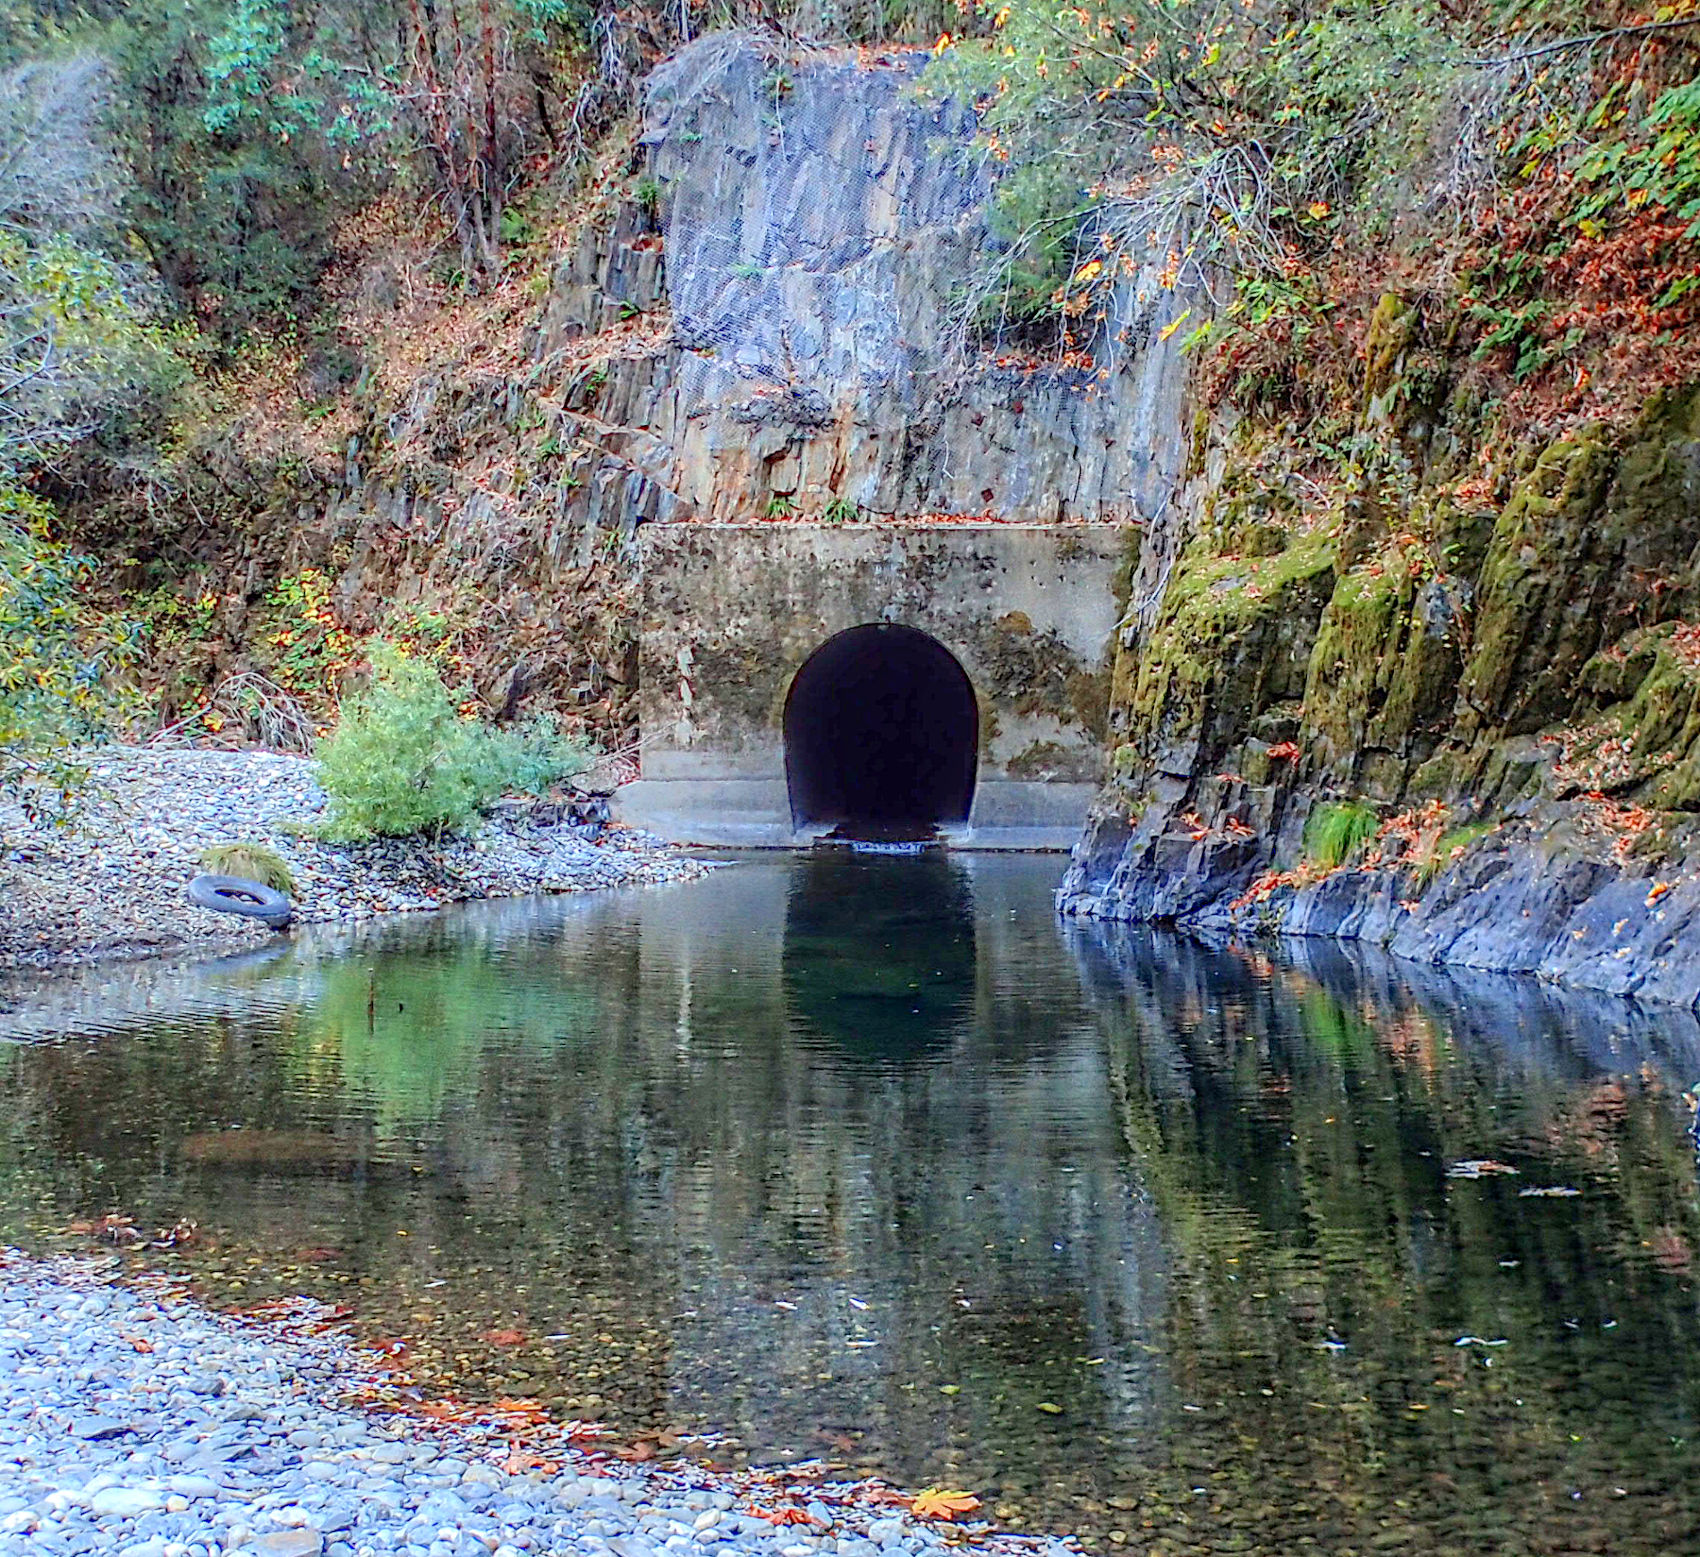
\includegraphics[height=0.37\paperheight]{sediment-bypass-tunnel-log-cabin}};
		\end{scope}
	}
	\onslide<1-1>{
		\node[anchor=south west, xshift=0.33\paperwidth, yshift=2.1947cm, text=black, text width=0.5\paperwidth,align=left]{\tiny \textcolor{gray}{Source: Chamoun \textit{et al.} / SCCER-SoE (2018)}};}
\end{tikzpicture}
\end{frame}


